% !TeX spellcheck = de_DE
%

\documentclass[a4paper,twoside,openright,12pt]{book}
\usepackage[utf8]{inputenc}  %Kodna stran za Windows okolje, za linux je kodna stran latin2
\usepackage[slovene]{babel}    % pravila za slovensko deljenje besed
\usepackage{tikz}
\usetikzlibrary{tikzmark}
\usetikzlibrary{shapes,arrows,positioning,calc,babel}
\usepackage[europeanresistors]{circuitikz}
\usepackage{graphicx}
\usepackage{psfrag}
\usepackage{epstopdf}
\epstopdfsetup{update}
\usepackage[pdftex]{UNI-LJ-FE-Diploma} %Stil za diplome na Fakulteti za elektrotehniko (za pdfTeX v MkiTex)
\usepackage{MojiBloki}
%\usepackage[pctex]{UNI-LJ-FE-Diploma} %Stil za diplome na Fakulteti za elektrotehniko  (za pcTex)
\usepackage{pgfplots}
\usepackage{subfigure} 
\usepackage{verbatim}
\usepackage{transparent}
\usepackage{tikz-timing}
\usetikztiminglibrary[rising arrows]{clockarrows}
\usetikztiminglibrary{arrows}
\usepackage{makecell}%
\usetikzlibrary{babel}
\usepackage{setspace}
\usetikzlibrary{math,calc}
%*************************** PRILAGODITVE *****************************
% mapa s slikami
\potgrafike{./Slike/}
\graphicspath{./Slike/}
%prilagoditev levega roba sodih strani. če se pri dvostranskem tisku robovi ne umemajo se lahko poveča ali pomanjča
\zamaknirobsodihstrani{0mm}

%*************************** NASLOVNA STRAN *****************************
\naslov{Navodila in predloga za izdelavo diplomskega in magistrskega dela}
\avtor{Marko Buršić} \univerza{Univerza v Ljubljani}
\fakulteta{Fakulteta za elektrotehniko}
\delo{Diplomsko delo}
%\delo{Diplomsko delo visokočolskega strokovnega čtudija}
\date{Ljubljana, 2016}
\mentor{prof. dr. Damijan Miljavec}
%\somentor{prof. dr. Ime Priimek}
\begin{document}
\graphicspath{{./slike/}}
%------------------------ ZAčETNI DEL -----------------------------------
\frontmatter
%------------------------------------------------------------------------
%
%************************ NASLOVNA STRAN ********************************

\maketitle


%*************************** ZAHVALA ************************************
\zahvala V zahvali se kandidati zahvali mentorju in poimensko tudi
vsem sodelavcem in prijateljem, ki so pomagali in prispevali pri
delu v laboratoriju, na računalniku, v delavnici, pri tehnični
izdelavi dela in drugje.








%*************************** VSEBINA *************************************
\tableofcontents

%*************************** SEZNAM SLIK in TABEL  ***********************
\seznamslik
\seznamtabel

%***************************  SEZNAM UPORABLJENIH SIMBOLOV  **************

\seznamsimbolov

V pričujočem zaključnem delu so uporabljeni naslednje veličine in
simboli:

\begin{table}[h]
\centering
%\begin{footnotesize}
\begin{tabular}{l l l l}
 \hline \multicolumn{2}{c}{\bf{Veličina / oznaka}} & \multicolumn{2}{c}{\bf{Enota}}  \\
 \hline
Ime & Simbol & Ime & Simbol \\
 \hline
 čas & $t$  & sekunda & s \\
 frekvenca & $f$  & Hertz & Hz \\
 obodna hitrost & $\omega$ & - & rad/s\\
 hitrost	& $v$ & - & m/s\\
 kotni pospešek & $\alpha$ & - & rad/s$^2$ \\
 linearni pospešek & $a$ & - & m/s$^2$ \\
 sila & $F$ & Newton & N\\
 masa   & $m$  & kilogram & kg \\
 moment   & $M$  & Newtonmeter & Nm\\
 vztrajnostni moment & $J$ & - & kgm$^2$ \\
 napestost & $U$ & Volt  & V \\
 tok	& $I$	&	Ampere & A\\
 upornost & $R$ & Ohm  & $\Omega$ \\
 prevodnost & $G$ & Siemens & S \\
 induktivnost & $L$ & Henry & H\\
 kapacitivnost & $C$ & Farad & F \\
 gostota magnetnega pretoka   & $B$  & Tesla & T\\
 jakost magnetnega polja   & $H$  & - & A/m\\
 nekaj   & $ $  & - & -\\
  \hline
\end{tabular}
%\end{footnotesize}
  \caption{Veličine in simboli}
  \label{prebojne_trdnosti}
\end{table}

Pri čemer so vektorji in matrike napisani s poudarjeno pisavo.
Natančnejči pomen simbolov in njihovih indeksov je razviden iz
ustreznih slik ali pa je pojasnjen v spremljajočem besedilu, kjer je
simbol uporabljen.


%------------------------ GLAVNI DEL ------------------------------------
\mainmatter
%-------------------------------------------------------------------------


%********************* POVZETEK V SLOVENččINI ****************************
\povzetek

V pričujočem delu so predstavljena navodila za izdelavo zaključnega
dela na Fakulteti za elektrotehniko v Ljubljani. Zaključno delo
predstavlja diplomsko delo na prvi stopnji ter magistrsko delo na
drugi stopnji izobračevalnega programa.

V povzetku v slovenččini in v angleččini kandidat navede glavne
rezultate dela, zato naj povzetek seznani bralca z jedrom dela na
način, ki je običajen za pisanje krajčih člankov ali referatov.
Obseg povzetka je za Repozitorij Univerze v Ljubljani omejen na tisoč
znakov.

Povzetek se naj prične z opisom in definicijo problema. Nadaljuje se
naj z opisom uporabljenih metod in postopkov, ki so privedli do
rečitve. Na koncu naj bodo opisani rezultati dela in glavni zaključki, ki iz rezultatov
izhajajo.

Za tem se na isti strani navede če ključne besede v slovenččini in v
tujem jeziku.

\kljucnebesede beseda1, beseda2, beseda3


%*************************** POVZETEK V ANGLEččINI ***********************
\abstract

The thesis addresses ...

\keywords word1, word2, word3


%***************************** UVOD **************************************
\chapter{Uvod} \label{uvod}

Uvod v zaključno delo ima namen, da uvede bralca v tematiko
zaključnega dela. V njem kandidat razčleni zahteve in cilje
zaključnega dela, po literaturi povzame znane rečitve in oceni
njihov pomen za zaključno delo. Sklicevanje na literaturo se v
besedilu označi s čtevilko v oglatem oklepaju, ki jo ima ta v
seznamu uporabljenih virov, in po potrebi navede strani, npr.
\cite{miklavvcivc2010objavljanje} 
%*********************** OSREDNJA POGLAVJA ********************************


\chapter{Dajalniki pozicije} \label{Dajalniki pozicije in hitrosti}
\section[Hall senzor]{Hall senzor}
Hall-ov pojav je posledica toka skozi prevodnik, ki se nahaja v magnetnem polju. Slika \ref{Hall_element.jpg} prikazuje tanek sloj prevodnika (Hall element) skozi katerega teče tok v smeri x-osi. Priključne sponke izhodnega signala se nahajajo na obeh robovih elementa na y-osi,  zunanje magnetno polje pa deluje v smeri z-osi. V kolikor zunanje magnetno polje ni prisotno, se elektroni pomikajo vzdolž x-osi v ravni smeri in na izhodnih sponkah ni zaznati razlike napetosti. V primeru prisotnosti zunanjega magnetnega polja, ki je pravokotno na smer gibanja elektronov le-ti občutijo t.i. Lorenz-ovo silo, ki povroča ukrivljanje smeri tako, da se na eni strani nabirajo elektroni, na drugi pa vrzeli in tako je možno izmeriti napetost  $V_H$ , kot razliko v potencialu med obemi robovi elementa. \cite{manual-Honeywell}

\bitnaslika{Osnovna zgradba Hall elementa}{Hall_element.jpg}{7cm}{6cm}

Napetost $V_H$ je premosorazmerna produktu toka skozi element in gostoto magnetnega pretoka.

\begin{equation}V_H \propto I\times B\end{equation}

Hall sensorje odlikuje jih velika robustnost, hitra odzivnost ter nizka cena zato imajo veliko uporabo v industrijski elektroniki, kot naprimer tokovni merilniki, senzorji prisotnosti,...itd v brezkrtačnih enosmernih motorjih se jih uporablja kot absolutne dajalnike pozicije rotorja, v absolutnih dajalnikih pozicije pa kot dekodirniki števca obratov. V nadaljevanju se bomo osredotočili le na uporabo senzorjev kjer nas analogna vrednost gostote magnetnega pretoka ne zanima, pač pa samo pristonost le-tega. V ta namen je potrebno preoblikovati  izhodno napetost  $\textbf{\textit{V}}_H$ v digitalen signal.

\bitnaslika{Hall senzor z digitalnim izhodom}{HALL_DIG.JPG}{7cm}{5cm}
Na sliki \ref{HALL_DIG.JPG} je prikazana zgradba senzorja z digitalnim izhodom vklopljeno/izklopljeno. Diferencialna napetost hall-ovega elementa je naprej ojačana z uporabo operacijskega ojačevalnika in nato preoblikovana v digitalen izhod s pomočjo schmitt triggerja, ki poskrbi za ustrezno histerezo med obemi stanji izhoda.  Glede na delovno področje histereze sta možna dva tipa: unipolarni in bipolarni. 

\bitnaslika{Primerjava med unipolarno in bipolrano obilko histereze}{HAll_histereza.png}{15cm}{6cm}
Unipolarni tip je namenjen za senzorje za zaznavo prisotnosti magnetnega pretoka, bipolarni pa je namenjen zaznavi prehoda magnetnih polov in je zato primeren kot sestavni del dajalnika pozicije.
\section[Resolver]{Resolver}
Resolver imenujemo v žargonu tudi rotirajoči transformator, je zelo robusten in cenovno zelo ugoden način merjenja kotne pozicije in hitrosti, . V primerjavi z ostalimi dajalniki pozicije ima resolver določene prednosti kot so: 
\begin{itemize}
	\item zmožnost delovanja v izjemno težkih okoljskih pogojih, kot so prah, vlaga in visoka temperatura  
	\item so izjemno mehansko odporni na udarce in pospeške 
	\item delujejo tudi pri zelo visoki vrtilni hitrosti brez izgube natančnosti   
\end{itemize}
Zaradi teh odličnih lastnosti ima veliko uporabo v vojaški in letalski tehniki ter v industrijskih servo pogonih kot absolutni dajalnik pozicije rotorja motorja. Seveda imajo tudi slabe lastnosti kot so: slabša natančnost primerljiva z optičnimi enkoderji, potrebuje zelo hiter AD pretvornik in zmogljiv procesor, ki pretvori analogno obliko signala v digitalno obliko pozicije in hitrosti.
\begin{figure}[h]
	\begin{center}
		\begin{circuitikz} \draw
			(0,0) node[transformer] (T) {}
			(T.A1) node[anchor=east] {}
			(T.A2) node[anchor=east] {}
			(T.B1) to[short] (2,0) 
			to [L, l=\textit{Rotor}] (4, -2.0)
			to [short] (4,-2.1)
			to [short] (T.B2)
			(T.base) node{K}
			
			[short] (7,0)
			to [short] (5,0)
			to [L, l =\parbox{3cm}{Stator\\ K $u_{vzb}$ cos $\Theta$}] (5,-2)
			to [short] (7,-2)
			
			[short] (2,-5)
			to [short] (2,-3)
			to [L, l_=\parbox{3cm}{Stator\\K $u_{vzb}$ sin $\Theta$}] (5,-3)
			to [short] (5,-5);
			\draw[dashed] (4.1,-2) -- ($(4.1,-2)!1.2!(2.1,0)$) 
			node[above,text width=2cm] {Kot rotorja ($\Theta$)}
			(4.1,-2) -- (4.1,1);
			\draw[->] (4.1,1) arc[start angle=90, end angle=135, radius=3]
			node[midway,below right] {$\theta$};
			\draw[<-] (T.south) -- ++(0,-0.5) node[below,text width=3cm] {Zračna reža};
		\end{circuitikz}
	\end{center}	    
	\caption{Zgradba resolverja}
	\label{fig:resolver_trafo}
\end{figure}

Na sliki \ref{fig:resolver_trafo} je prikazana osnovna zgradba resolverja. Na statorju se nahajajo vzbujalno navitje ter dve navitji iz katerih dobimo povratni signal sin in cos. Skozi primarno navitje transformatorja je pritisnjena sinusna vzbujalna napetost, katera inducira tok v sekundarnem (rotorskem) tokokrogu, ki je v fazi s primarnim tokom in nedovisen od položaja rotorja in teče skozi drugo navitje rotorja, ki ima izražene pole. Rotorski tok, inducira napetost  v statorskih navitjih sin in cos, ki sta geometrično zamaknjeni za 90 stopinj. Zaradi izraženosti polov rotorja in geometrične postavive sin cos navitij, so napetosti odvisni od položaja rotorja. Običajna vrednost amplitude vzbujalne napetosti $U_{vzb}$ je 1$V_{pp}$, frekvenca pa se giblje nekje med 1-10kHz.
\begin{equation} \label{resolver_uvzb}
u_{vzb} = U_{vzb}\;sin\omega t
\end{equation}

\begin{equation} \label{resolver_uout}
\begin{aligned}
	u_{cos} = K\;u_{vzb}\;cos\Theta \\ 
	u_{sin} = K\;u_{vzb}\;sin\Theta 
\end{aligned}
\end{equation}


V enačbah \ref{resolver_uout} sta prikazana odvisnonst napetetosti med sin in cos navitjema ter vzbujalno napetostjo resolverja,  na sliki \ref{fig:resolver_signali} pa tudi njihov potek.

\begin{figure}[h]
	\begin{center}	
		\pgfplotsset{width=10cm,compat=1.13}	
		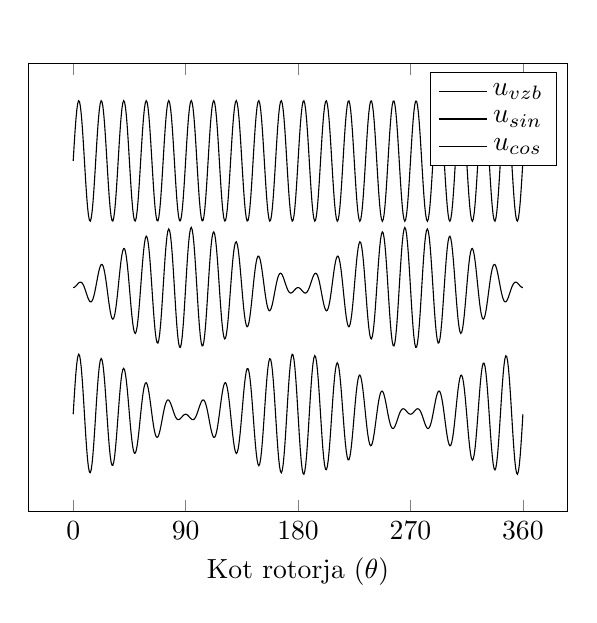
\begin{tikzpicture}
		\begin{axis}[
		title=\empty,
		xlabel={Kot rotorja ($\theta$)},
		ytick=\empty,
		xtick={0,90,180,270,360},
		]
		\addplot[samples=500,domain=0:360]{sin(20*x)+4.2};
		\addplot[samples=500,domain=0:360]{sin(20*x)*sin(x)+2.1};
		\addplot[samples=500,domain=0:360]{sin(20*x)*cos(x)};
		
		\legend{$u_{vzb}$,$u_{sin}$,$u_{cos}$}
		\end{axis}
		\end{tikzpicture}
		  \caption{Napetostni signali resolverja}
		  \label{fig:resolver_signali}
	\end{center}		  
\end{figure}


\begin{equation} \label{resolver_theta}
\begin{aligned}
\frac{u_{sin}}{u_{cos}} & = \frac{K\;u_{vzb}\;sin\Theta }{K\;u_{vzb}\;cos\Theta } =\frac{sin\Theta}{cos\Theta} =\tan\Theta \\[10pt]
\Theta & = \arctan(\frac{u_{sin}}{u_{cos}})
\end{aligned}
\end{equation}

Konstanta K je sklopni faktor, odvisen je od velikosti reže ter razmerja ovojev med primarjem in sekundarjem. Ta podatek je pomemben pri izbiri resolverja z že podanim AD pretvornikom, saj le-ti imajo merilno območje prilagojeno prav na sklopni faktor K. Iz enačbe \ref{resolver_theta} je razvidno, da padec napetosti zaradi ohmske upornosti, kot tudi različen sklopni faktor nimajo nikakršnega vpliva na točnost meritve vse dokler je povraten signal v merilnem območju AD pretvornika, to dosežemo z izborom resolverja, kateri ima ustrezen sklopni faktor.\\
Kot rotorja $\Theta$ se lahko izračuna na preprost način, kot prikazano v enačbi \ref{resolver_theta}, ta metoda je najbolj natančna, če se vzorci signala zajemajo v točki maksimalne napetosti. Poleg rotorskega kota je zaželjeno, da nam dajalnik podaja tudi hitrost, zato so se razvile različne metode, ki so bolj natančne in izračunajo tudi hitrost. Novejša metoda v uporabi se imenuje sledenje opazovanega kota (\textit{angl. Angle Tracking Observer}). Blokovna shema metode prikazana na sliki \ref{resolver1}, temlji na zaprtozančnem sistemu, pri čemer primerjamo signala resolverja $u_{sin}$ in   $u_{cos}$ z njihovima približkoma. Podobno kot pri vskem zaprtozančnem sistemu je smisel čimbolj zmanjšati statični pogrešek. Pogrešek opazovanega kota je razlika med pravim kotom $\Theta$ in  približkom $\hat{\Theta}$ \cite{Reddy-ATO}. Za izračun pogreška z danima signalima  $u_{sin}$ in   $u_{cos}$ se poslužujemo svojstva trigonometrične funkcije $\sin(\Theta - \hat{\Theta}) =  \sin\Theta\;\cos\hat{\Theta} -  \cos\Theta\;\sin\hat{\Theta}$ in njena realizacija se na sliki \ref{resolver1} vidi kot vhodni signal v ojačevalnik $K_1$. Sedaj  bi lahko sledil logičen sklep, da je potrebno izračunati še inverzno trigonometrično funkcijo $\arcsin$, če želimo dobiti razliko $\Theta - \hat{\Theta}$. Ponovno izrabimo svojstvo trigonometrične funkcije in zapišemo, da za majhne odmike velja  $\sin(\Theta - \hat{\Theta}) \approx \Theta - \hat{\Theta} $. Sistem sledenja sestoji iz integratorja in PI regulatorja, prenosna funkcija zaprte zanke je prikazana v enačbi \ref{resolver_trfcn1}, nadalje pa se za lažjo predstavo prenosno funkcijo opiše kot člen drugega reda, pri čemer je $\omega_{n}$ lastna frekvenca, $\xi$ pa faktor dušenja \cite{semiconductor2009using}. Ustrezna izbira parametrov omogoča odziv na enotino stopnico tako, da ima izhodni signal čim hitrejši odziv s čim manjšim prenihajem.
\begin{figure}[h]
	\centering

%	\includegraphics[width=0.75\columnwidth]{resolver4}
	 \def\svgwidth{\columnwidth}
	 \input{Slike/resolver5.eps_tex}
	 \caption{\label{resolver1} Blokovna shema metode Angle Tracking Observer}
\end{figure}
\begin{equation} \label{resolver_trfcn1}
H(s) = \frac{\hat{\Theta}}{\Theta} = \frac{K_{1}(1+K_{2}s)}{s^{2}+K_{1}K_{2}} 
\end{equation}
\begin{equation} \label{resolver_trfcn2}
H(s) = \frac{\omega_{n}^{2}(1+2\xi s/\omega_{n})}{s^{2}+2\xi\omega_{n}s+\omega_{n}^{2}} \approx\frac{\omega_{n}^{2}}{s^{2}+2\xi\omega_{n}s+\omega_{n}^{2}}
\end{equation}
\begin{equation} \label{resolver_trfcn3}
\begin{aligned}
K_{1} & =\omega_{n}^{2}\\[5pt]
K_{2} & =\frac{2\xi}{\omega_{n}}
\end{aligned}
\end{equation}
\section[Optični inkrementalni dajalnik]{Optični inkrementalni dajalnik}
\begin{figure}[h]
	\centering
	\includegraphics[width=0.5\columnwidth]{Enkoder_delovanje}
	\caption{\label{inkr_enkoder_del} Poenostavljena zgradba inkrementalnega dajalnika}
\end{figure}
Optični inkrementalni dajalnik je najbolj pogosto uporabljen pozicijski dajalnik v elektromotornih pogonih. Njegove dobre lastnosti so natančnost in relativno nizek strošek izdelave, kot slabosti pa štejemo: občutljivost na mehanske poškodbe, omejena življenska doba zaradi slabljenja občutljivosti foto detektorjev, omejena vrtilna hitrost delovanja zaradi omejene preklopne frekvence foto detektorjev. Na sliki \ref{inkr_enkoder_del} je prikazana poenostavljena zgradba inkrementalnega dajalnika: izvor svetlobe, disk z optično rešetko iz naparjene kovine, uklonska mrežica in foto detektorji. Svetlobni tok pronica skozi rotorsko rešetko in uklonsko mrežico do foto detektorjev A in B proge, ki sta zamaknjena za 90$^\circ$  glede na modulirano svetlobo, le-ta nastane zaradi uklona svetlobe pri pehodu skozi dve rešetki, kateri imata različen raster. Ta pojav se imenuje Moire-jev vzorez in na sliki \ref{moire} \cite{gabrielyan2007basics} je prikazan pomik rotorskega diska za en razdelek glede na statorsko ploščo, kjer se lepo vidi zatemnjene in osveltjene dele. Z uporabo uklonske mrežice je možno ustvariti ustrezno velika področja zatemnitve, da jih lahko foto detektor zazna, navkljub svoji večji fizični velikosti od samega rasterja rotorske plošče. Jakost svetlobe ima sinusno obliko v območju pomika za en razdelek (raster) in jo lahko pretvorimo v električni signal tako, da uporabimo za vsako progo dva fotodetektorja, ki sta zamaknjena za 180$^\circ$, imenujemo jih $A$,$\bar{A}$ ter $B$,$\bar{B}$. Njihove signale ojačamo z diferencialnim ojačeavlanikom, kot prikazano na sliki \ref{inkr_enkoder_diffamp}, tako dobimo na izhodu diferencialnega ojačevalnika sinusni signal katerega nato preoblikujemo v pravokotne pulze, ki so primerne oblike za štetje z digititalnim števcem. Na sliki \ref{inkr_enkoder_izhod} so prikazani izhodni signali dveh prog in ponazoritev impulzov števca v pozitivno in negativno stran iz katerega tudi izhaja ime: inkrementalni dajalnik. Prikazani način štetja se v literaturi imenuje $4\times$, ker se v števec prišteva ob vsakem prehodu signala bodisi proge $A$ ali $B$, zato je število pulzov na en obod enako štirikratniku števila črtic, ki jih ima rotorski disk. Primer rotorskega diska na sliki \ref{inkr_enkoder1} ima 128 črtic, kar bi naneslo 512 pulzov števca na en obrat. Pridobljena pozicija je tako relativen pomik od referenčne točke, ki jo je ob vsakem ponovnem zagonu potrebno znova določiti, saj inkrementalni dajalnik nam ne daje absolutne pozicije. 
\begin{figure}[h]
	\centering
	\includegraphics[width=0.35\columnwidth]{inkr_enkoder1}
	\caption{\label{inkr_enkoder1} Disk inkrementalnega enkoderja}
\end{figure}
\begin{figure}    
	\begin{minipage}[t]{0.3\textwidth}
		\includegraphics[width=\linewidth]{moire-a}
	\end{minipage}	
	\hspace{\fill}	
	\begin{minipage}[t]{0.3\textwidth}
		\includegraphics[width=\linewidth]{moire-b}
	\end{minipage}
	
	\vspace*{0.5cm} % (or whatever vertical separation you prefer)	
	\begin{minipage}[t]{0.3\textwidth}
		\includegraphics[width=\linewidth]{moire-c}
	\end{minipage}	
	\hspace{\fill}
	\begin{minipage}[t]{0.3\textwidth}
		\includegraphics[width=\linewidth]{moire-d}
	\end{minipage}
	\caption{\label{moire}Uklon na mrežici}
\end{figure}
\begin{figure}[h]
	\centering
	\begin{tikztimingtable}
		PROGA A   & SS H 4{LLHH} HHHH 3{LLHH} L  \\ % ends with edge
		PROGA B   & SS  4{LLHH} LL 4{LLHH} L \\ % starts with edge
		ŠTEVEC 4$\times +$ & SSS 16{A}   \\ % ends with edge
		ŠTEVEC 4$\times -$ & SS 20{S} 15{A}   \\ % ends with edge
	\end{tikztimingtable}
	\caption{\label{inkr_enkoder_izhod} Izhodni signali inkrementalnega enkoderja}
\end{figure}
\begin{figure}[h]
	\begin{circuitikz}  
		\draw  (6,4) node[op amp] (opamp) {}  
		(0.0,1.5) to  [pDo, l=$fotodetketor \bar{A}\;\;\;$]  (0.0,4.5)
		(2.0,1.5) to  [pDo, l=$fotodetketor A\;\;$]  (2.0,3.5)	
		(2,3.5) to [short, l=$V_A$] (3,3.5)  
		(0,1.5) to [short, -o] (8,1.5)  
		(0,4.5) to [short,l=$V_{\bar{A}}$] (3,4.5)  
		(3,4.5) to [R, l=$R_a$]  (4.5,4.5)  
		(4.5,4.5) to [short,-*] (4.8,4.5) 	
		(4.8,3.5) to [R, l=$R_g$] (4.8,1.5)  
		(4.8,1.5) to [short,*-*] (4.8,1.5)  
		(4.8,3.5) to [short,*-*] (4.8,3.5)
		(3,3.5) to [R,l_=$R_a$] (4.5,3.5)  
		(4.5,3.5) -- (opamp.+) 
		(5.2,5.5) to [R, l=$R_g$] (7.2,5.5) 
		(7.2,5.5) to [short,-*] 
		(opamp.out) (6.8,4) to [short,-o] (8,4)  
		(opamp.-) -- (4.8,5.5)  
		(4.8,5.5) -- (4.8,5.5) -- (5.2,5.5)  ;  
		\draw[->] (7.75,3.8) to node[right] {$V_{izhod}=(V_A-V_{\bar{A}})\frac{R_g}{R_a}$} (7.75,1.7);
	\end{circuitikz}
	\caption{\label{inkr_enkoder_diffamp} Diferencialni ojačevalnik ima na izhodu sinusni signal}
\end{figure}
\subsection{Meritev hitrosti z inkrementalnim dajalnikom}
Pri pozicioniranju elektromotornih pogonov je poleg pozicije, pomembna tudi informacija o hitrosti.  
Ker je inkrementalni dajalnik po svoji zasnovi merilnik položaja se lahko hitrost meri posredno iz spremembe položaja v merilnem intervalu kot meritev periode pulzov ali kot meritev frekvence pulzov inkrementalnega dajalnika. 
\subsubsection{Metoda merjenje frekvence}
Na sliki \ref{inkr_enkoder_metoda_f} je prikazana metoda merjenja frekvence. Pulzi iz števca pozicije se merijo v fiksnih intervalih $T_{vz}$, le-ta je določen glede na periodo vzorčenja regulacijske zanke (gl. poglavje xx). Iz prikaza je razvidno, da pri nizki frekvenci pulzov postane metoda nenetančna, kot vidimo je število preštetih pulzov $N_f$ pri isti vhodni frekvenci v zaporednih merilnih intervalih različno: 2, 2, 3, 2. Enačba \ref{inkr_enkoder_omega_metodaf} opisuje preračunano hitrost $\Omega_f$ \cite{vcurkovivcmeritev}, pri čemer je faktor 4 v enačbi posledica štetja vhodnih pulzov po metodi  $4\times$ opisani na sliki \ref{inkr_enkoder_izhod}. Relativni pogrešek $e_f$ \cite{bergelj1993osnove} metode je odvisen od dolžine periode merjenega signala $T_p$. Pri večanju periode vhodnega signala postaja pogrešek čedalje večji, kar pomeni da lahko to metodo uporabimo le pri visoki frekvenci vhodnih pulzov.
\begin{figure}[h]
	\centering
	\begin{tikztimingtable}
		pulzi   &  SS 12{1.7A}  \\ % ends with edge
		merilni interval  &   SSSSASSSASSSASSSASSSA \\
		1. meritev  &  SS 2{1.7S} 2{1.7A}   \\
		2. meritev  &  SS 4{1.7S} 2{1.7A}   \\ 
		3. meritev  &  SS 6{1.7S} 3{1.7A}   \\ 	
		4. meritev  &  SS 9{1.7S} 2{1.7A}   \\ 	
		\\
		\extracode
		% Add vertical lines in two colors
		\begin{pgfonlayer}{background}
			\begin{scope}[semitransparent,semithick]
				\vertlines[red]{4,8,13.9,15.6}
				\horlines{1,2,3,4,5,6}
			\end{scope}
		\end{pgfonlayer}	
		\draw[<->, thick, black](4,-12) -- (8,-12);
		\draw[<->, thick, black](13.9,-12) -- (15.6,-12);
		\node[align=center, below] at (6,-12) {$T_{vz}$};
		\node[align=center, below] at (15,-12) {$T_{p}$};
		\node[] at (25,-3) {$N_f=2$};
		\node[] at (25,-5) {$N_f=2$};
		\node[] at (25,-7) {$N_f=3$};
		\node[] at (25,-9) {$N_f=2$};
	\end{tikztimingtable}
	\caption{\label{inkr_enkoder_metoda_f}Metoda merjenja frekvence}
\end{figure}
\begin{equation} \label{inkr_enkoder_omega_metodaf}
\begin{aligned}
\Omega_f & =\frac{2\pi N_f}{4N_{crtic}T_{vz}}\\[5pt]
e_f & =\pm\frac{T_p}{T_{vz}}=\pm\frac{1}{N_f}
\end{aligned}
\qquad\qquad\parbox{4.0cm}{\footnotesize$
	\begin{aligned} 
	N_{crtic} & \quad \text{število črtic na rotorski plošči}\\[-1.0ex] 
	N_f & \quad \text{število preštetih pulzov}\\[-1.0ex] 
	T_p & \quad \text{perioda merjenega signala}\\[-1.0ex]
	T_{vz} & \quad \text{čas vzorčenja}\\[5pt]
	\end{aligned}$}
\end{equation}
\subsubsection{Metoda merjenje periode}
Naslednja metoda, katera je primerna za merjenje hitrosti meri čas periode vhodnih pulzov namesto frekvence, zato je primerna za merjenje pri nizkih hitrostih. Med dvema zaporednima pulzoma merjenega signala štejemo pulze urinega takta. Izbrana frekvenca urinih pulzov je najvišja možna glede na dane zmožnosti elektronske merilne enote, saj se relativni pogrešek  $e_T$ manjša ob večanju frekvence urinega takta. Enačba \ref{inkr_enkoder_omega_metodaT} opisuje izračun hitrosti $\Omega_T$ glede na število preštetih pulzov $N_T$ ter periode urinih pulzov $T_{ure}$.
\begin{figure}[h]
	\centering
	\begin{tikztimingtable}
		pulzi   &  SSASSSSSSSSSSA  \\ % ends with edge
		ura  &   C 22{0.9C}\\
		meritev &  3{0.9S} 6{1.8A} \\
		\\
		\extracode
		% Add vertical lines in two colors
		\begin{pgfonlayer}{background}
			\begin{scope}[semitransparent,semithick]
				\vertlines[red]{2,13,15.4,17.2}
				\horlines{1,2,3}
			\end{scope}
		\end{pgfonlayer}	
		\draw[<->, thick, black](2,-6) -- (13,-6);
		\draw[<->, thick, black](15.4,-6) -- (17.2,-6);
		\node[align=center, below] at (10,-6) {$T_p$};
		\node[align=center, below] at (16.5,-6) {$T_{ura}$};
		\node[] at  (23,-3.2) {$N_{T}=6$};
	\end{tikztimingtable}
	\caption{\label{inkr_enkoder_metoda_T}Metoda merjenja periode}
\end{figure}
\begin{equation} \label{inkr_enkoder_omega_metodaT}
\begin{aligned}
\Omega_T & =\frac{2\pi}{4N_{crtic}N_{T}T_{ure}}\\[5pt]
e_T & =\pm\frac{T_{ure}}{T_p} =\pm\frac{1}{N_T}
\qquad\end{aligned}
\qquad\parbox{4.0cm}{\footnotesize$
	\begin{aligned} 
	N_{crtic} & \quad \text{število črtic na rotorski plošči}\\[-1.0ex] 
	N_T & \quad \text{število preštetih pulzov}\\[-1.0ex] 
	T_p & \quad \text{perioda merjenega signala}\\[-1.0ex]
	T_{ure} & \quad \text{perioda urinih pulzov}\\[5pt]
	\end{aligned}$}
\end{equation} 
\subsubsection{Kombinirana metoda merjenja frekvence in periode}
Ker metodi merjenja frekvence ali periode same po sebi ne zagotavljata točnost meritve na širokem obsegu hitrosti, je smiselno združiti obe v kobinacijo le-teh. Kot prikazano na diagramih poteka, bi lahko za posamezne metode uporabili zgolj logična vrata, nekaj bistabilnih multivibratorjev in urin takt z zelo visoko frekvenco. Vsi ti elementi se lahko sprogramirajo v logično enoto z uporabo FPGA logike, ki meri hitrost po obeh metodah in preklaplja rezultat glede na relativni pogrešek obeh. Če pogledamo enačbi \ref{inkr_enkoder_omega_metodaf} un \ref{inkr_enkoder_omega_metodaT} nam je takoj jasno, da je za izbiro ugodnejše metode dovolj primerjava preštetih pulzov $N_f$ in $N_T$.
\subsection{Sin/Cos inkrementalni dajalnik }
Sin/Cos dajalnik se v sami zgradbi ne razlikuje on inkrementalnega, razlika je le v izhodnem signalu dajalnika. Kot smo spoznali, daje inkrementalni dajalnik provokotne pulze, ki so bili predhodno preoblikovani iz sinusne napetosti, ki jo daje diferencialni ojačevalnik prikazan na sliki \ref{inkr_enkoder_diffamp}. Sin/Cos dajalnik posreduje izhoden signal, ki je ravno takšne sinusne oblike z amplitudo $1V_{pp}$ za progo $A$ in $B$, ki sta medseboj zamaknjeni za 90$^\circ$, se pravi sinus in kosinus, od tod ime Sin/Cos. Ta dva signala peljemo do vhoda merilne enote pozicije (slika \ref{EnkoderSinCos}, \cite{schmirgel2009fpga}), kjer se razdelita na dva dela. V prvem delu se signala preoblikujeta v pravokotne pulze in preštevajo po že omenjenih metodah. Drugi del sestoji iz računala, ki preračunava vmesni kot med dvemma črticama na rotorskem disku in na tak način z interpolacijo vrine še dodatne vmesne točke pozicije. Metoda izračuna kota se v bistvu ne razlikuje od že opisane medote  \textit{Angle Tracking Observer}. Prednosti Sin/Cos dajalnika je v tem, da je možno izračunati že zelo majhno hitrost in obenem je tak dajalnik uporaben tudi za visoke vrtilne hitrosti, saj potrebuje manjše število črtic na disku v primerjavi z inkrementalnim dajalnikom za isto resolucijo, kar posledično pomeni nižjo frekvenco preklapljanja fotodetektorjev, katera je omejena z vidika tehnoloških zmožnosti fotodetektorja. Tak tip dajalnika srečamo na CNC strojih za obdelavo kovine, kjer je zahtevana največja natančnost.
\begin{figure}[h]
	\centering
	\includegraphics[width=0.5\columnwidth]{EnkoderSinCos}
	\caption{\label{EnkoderSinCos} Merilna enota Sin/Cos enkoderja }
\end{figure}
\section{Absolutni optični dajalnik}
\begin{figure}[h]
	\centering
	\includegraphics[width=0.35\columnwidth]{Absolutni_enkoder_disk}
	\caption{\label{EnkoderSinCos} Disk absolutnega enkoderja 10 prog}
\end{figure}
Absoultni optični dajalnik se razlikuje od inkrementalnega po tem da ima več prog in nam podaja absoultno pozicijo za en obrat rotorja. Za $2^N$ pozicij je potrebnih $N$ prog, katere so razvrščene po Gray-evi kodi. Gray koda je oblika binarnega zapisa, kjer se dve sosednji vrednosti razlikujeta le za en bit. Zasnovana oblika kodiranja je nastala kot ustrezna rešitev problema lažnih preklopev med stanji binarne kode. V binarni kodi namreč, bi se morala stanja vseh elektromehaskih preklopnikov spremeniti sinhrono ob vsakem novem stanju, to pa seveda v praksi ni mogoče. Iz tabele \ref{Absolutni_enkoder_disk_Gray} je ravidna razlika med binarno in Gray-evo kodo in sicer vsako novo stanje se v Gray kodi razlikuje od prejšnjega samo v enem bitu, puščice ponazarjajo redosled prehodov med stanji, ki ima lahko tudi obratno smer v primeru vrtenja dajalnika nazaj. Na sliki \ref{Absolutni_enkoder_disk_Gray} je prikaz oblike vzorca rotorske plošče absolutnega dajalnika. Absolutne dajalnike v kombinaciji z večobratnim števcem (gl. naslednje podpoglavje) se uporablja v strojih pri katerih je zaželjeno imeti znano pozicijo tudi v primeru izpada električne energije in povsod tam, kjer bi začetno iskanje referenčne točke povročalo težave. Primer takšnih strojev so dvigala, avtomatizirana regalna skladišča, proizvodna linija polizdelkov,...itd.
\begin{table}[h]
	\centering
	\begin{footnotesize}
		\begin{tabular}{|r|c||c|l|}
			\hline Decimalno &Binarno & Gray &  Gray v decimalni obliki\\
			\hline \hline
			0  & 0 0 0 & \tikzmark{j}0 0 0\tikzmark{a} &  0 \\
			1  & 0 0 1 & 0 0 1\tikzmark{b} &  1 \\
			2  & 0 1 0 & 0 1 1\tikzmark{c} &  3 \\
			3  & 0 1 1 & 0 1 0\tikzmark{d} &  2 \\
			4  & 1 0 0 & 1 1 0\tikzmark{e} &  6 \\
			5  & 1 0 1 & 1 1 1\tikzmark{f} &  7 \\
			6  & 1 1 0 & 1 0 1\tikzmark{g} &  5 \\
			7  & 1 1 1 & \tikzmark{i}1 0 0\tikzmark{h} &  4 \\
			\hline
		\end{tabular}
		\begin{tikzpicture}[overlay, remember picture, yshift=.25\baselineskip, shorten >=.5pt, shorten <=.5pt]
		 \draw [->] ({pic cs:a}) [bend left] to ({pic cs:b});
		 \draw [->] ({pic cs:b}) [bend left] to ({pic cs:c});
		 \draw [->] ({pic cs:c}) [bend left] to ({pic cs:d});
		 \draw [->] ({pic cs:d}) [bend left] to ({pic cs:e});
		 \draw [->] ({pic cs:e}) [bend left] to ({pic cs:f});
		 \draw [->] ({pic cs:f}) [bend left] to ({pic cs:g});
		 \draw [->] ({pic cs:g}) [bend left] to ({pic cs:h});
		 \draw [->] ({pic cs:i}) [bend left] to ({pic cs:j});  
		\end{tikzpicture}		
	\end{footnotesize}
	\caption{Primerjava prehoda stanj v binarni in Gray kodi}
	\label{Absolutni_enkoder_disk_Gray}
\end{table}

\section{Večobratni števec}
\bitnaslika{Primer zgradbe večobratnega mehanskega števca}{AbsolutniKodirniDisk.jpg}{7cm}{6cm}
Do sedaj opisana absoltuna dajalnika resolver in optični lahko podajata absolutno pozicijo le v območje enega obrata rotorja, vendar je to v praksi premajhno uporabno območje, zato se jim doda še večobratni števec. To je mehanska naprava, podobna števcu za porabo vode s to razliko, da je kodirana v Grey kodi in ima namesto cifer Hall senzorje za odčitavanje magnetnih prog, ki so nanešene na zobnikih. Na sliki \ref{AbsolutniKodirniDisk.jpg} je prikazana praktična izvedba takšnega števca, ki skupaj z absolutnim dajlinikom tvorita t.i. večobratni absolutni dajalnik. V podatkih proizvjalca \cite{temperature3sendix} se nahaja ločen podatek o tem kolikšna je resolucija na en obrat (npr. 10-bit = 512 razdelkov/obrat) ter kolikšen je obseg obratov (npr. 12-bit = 4096 obratov).
\chapter{Električni stroji}
Električni stroji so naprave s katerimi pretvarjamo energijo s posredovanjem magnetnega polja. To so elktromagnetne naprave, ki pretvarjajo električno energijo v mehansko energijo, mehansko energijo v električno energijo in električno energijo ene oblike v električno energijo druge oblike. Po svojem namenu uporabe so to električni mootorji, električni generatorji in transformatorji \cite{miljavec2009vezna} V nadaljevanju se bomo osredotočili le na električne stroje, ki imajo zmožnost pretvarjanja električne energije v mehansko in obratno ter so sklopljeni z mehanskim sistemom, z drugim imenom jih imenujemo elektromotorni pogoni.\\  
\begin{figure}[h]
	\begin{circuitikz}[european inductors]
		%\draw [help lines] (-1,-2) grid (12,5);
		
		% začetna črta
		\draw (0,3) to[R, o-, i>^=$I_q$, l=$R_q$] (3,3);
		\draw (3,3) to[L, l=$L_q$] (4,3);
		
		\draw (4,3) -- (5,3);
		\draw (5,3) to[V, v_=$U_i$] (5,0);
		%povratna črta
		\draw (5,0) to [short , -o]  (0,0);
		\draw[->] (0,2.8) to node[left] {$U_q$} (0,0.2);
		% rotor
		\draw[fill=black] (4.85,0.85) rectangle (5.15,2.15);
		\draw[fill=white] (5,1.5) ellipse (.45 and .45);
		%vzbujanje
		\draw (0.6, 0.5) to [short , o-,  i>^=$I_d$,] (0.6,1.5);
		\draw (0.6,1.5) to[R, l=$R_d$] (2.4,1.5);
		\draw (2.4,1.5) to[L, l=$L_d$] (3.8,1.5);
		\draw (3.8,1.5) to [short , -o] (3.8,0.5);
		\draw[->] (0.8,0.5) to node[above] {$U_d$} (3.6,0.5);
		%q,d-os
		%	\draw[dashed,->] (5,1.5)  to node[very near end, right] {$q-os$} (5,5) ;
		%	\draw[dashed,->] (5,1.5)  to node[very near end,above] {$d-os$} (13,1.5) ;
		
		% osovina iz motorja
		\draw[fill=black] (5.45,1.45) rectangle (7.8,1.55);
		% omega
		\draw[line width=0.7pt,<-] (5.8,1) arc (-30:30:1);
		% M
		\draw[line width=0.7pt,<-] (6.5,1) arc (-30:30:1);
		% vztrajnik
		\draw[fill=white] (8.5,1.49)
		ellipse (.15 and 0.4);
		\draw[fill=white, color=white] (7.9, 1.89)
		rectangle (8.49, 0.02);
		\draw (7.8,1.49) ellipse (.15 and 0.4);
		\draw (7.8,1.89) -- (8.5,1.89);
		\draw (7.8,1.09) -- (8.5,1.09);
		% Ja
		\draw[line width=0.7pt, ->] (7.2,1.0) arc (-30:30:1);
		% gred na bremenu
		\draw[fill=black] (8.65,1.45) rectangle (10.9,1.55);
		% zavora
		\draw[fill=black] (9.55,{0.53+1.07})
		-- +(-0.2,0.3) -- +(0.5,0.3) -- +(0.3,0.0);
		\draw[fill=black] (9.55,{0.33+1.07})
		-- +(-0.2,-0.3) -- +(0.5,-0.3) -- +(0.3,0.0);
		% Fomega
		\draw[line width=0.7pt,->] (9.05,1.0) arc (-30:30:1);
		
		% ML
		\draw[line width=0.7pt,->] (10.4,1.0) arc (-30:30:1);
		\draw (5.85,2.2) node {$\Omega$};
		\draw (6.5,2.2) node {$M$};
		\draw (7.29,2.2) node {$J\alpha$};
		\draw (9.0,2.2) node {$F\Omega$};
		\draw (10.4,2.2) node {$M_L$};
		\draw (8.25,1.51) node {$J$};
		
		\draw [decorate,decoration={brace,amplitude=10pt},
		xshift=0pt, yshift=0pt]
		(5.5,-0.75) -- (-0.5,-0.75)
		node[black,midway,yshift=-20pt]
		{električni stroj};
		\draw [decorate,decoration={brace,amplitude=10pt},
		xshift=0pt, yshift=0pt]
		(11.4,-0.75) -- (6,-0.75)
		node[black,midway,yshift=-20pt]
		{mehanski  sistem};
	\end{circuitikz}
	\caption{\label{DcMotor_predstava}Pogon s kolektorskim enosmernim tuje vzbujanim motorjem}
\end{figure}
Na sliki \ref{Pogon_moment_ravnovesje} je prikazan sklop elektromotornega pogona. Sestoji se iz električnega stroja in mehanskega sistema , ki sta medseboj povezana in med njima delujejo navori, ki so  v ravnovesju kot to opisuje ravnovesna enačba (\ref{Pogon_moment_ravnovesje}). Navorna ravnovesna enačba popisuje ravnotežje navorov, ki delujejo na gredi stroja in vplivajo na vrtenje rotorja. Poleg elekromagnetnega navora $M$ delujejo na gred še drugi navori, ki izvirajo iz mehanike samega stroja. Ob tem pa še navori, ki izvirajo iz zunanjih naprav priključenih na gred. Vsi ti navori morajo biti na gredi vsak trenutek obratovanja v ravnotežju. Posamezne oznake pomenijo: $\Omega$ je trenutna kotna hitrost vrtenja gredi in rotorja; $M$ je pogonski navor stroja; $M_L$ je zunanji bremenski navor, ki zavira vretnje gredi pri motorskem delovanju, negativna vrednost $M_L$ pomeni navor, ki poganja rotor v smeri vrtenja v generatorskem delovanju; $J\alpha$ je navor, ki izvira iz vztrajnostnega momenta $J$ vseh vrtečih se mas in skuša preprečiti vsako spremembo hitrosti $\Omega$; $F\Omega$ je navor viskoznega trenja, ki deluje vedno zaviralno ter ga je pogosto treba upoštevati pri obravnavi visoko dinamičnih pogonov \cite{miljavec2009vezna}.

\begin{equation} \label{Pogon_moment_ravnovesje}
\begin{aligned}
	0  &= M-J\alpha-F\Omega-M_L\\[5pt]
	J\alpha & = J\frac{d\Omega}{dt} = J\frac{d^2\Theta}{dt^2}=Js^2\Theta\\[5pt]
	F\Omega & = F\frac{d\Theta}{dt}=Fs^2\Theta\\[5pt]
\end{aligned}
%\qquad\qquad\parbox{4.0cm}{\footnotesize$
%	\begin{aligned} 
%	M & \quad \text{Pogonski elektromagnetni navor}\\[-1.0ex] 
%	J\alpha & \quad \text{navor zaradi vztrajnostnih mas}\\[-1.0ex] 
%	F\Omega & \quad \text{navor zaradi viskoznega trenja}\\[-1.0ex]
%	M_L & \quad \text{bremenski navor}\\[5pt]
%	\end{aligned}$}
\end{equation}
\section{Enosmerni kolektorski motor s tujim vzbujanjem}
Zaradi  dokaj enostavne možnosti regulacije enosmernega kolektorskega motorja s tujm vzbujanjem je dolgo let kraljeval v industriji kot servo pogon. Dandanes pa je  skoraj že povsem zamenjan z ostalimi motorji kot so na primer: sinhronski  servo motor s trajnimi magneti ali pa brezktraćni ennosmerni motor. Obstaja pa dejstvo, da je poznavanje delovanja enosmernega kolektorskega motorja pogoj za kasnejše razumevanje ostalih tipov motorjev, saj se je v letih uveljavil pristop pretvorbe rotirajočih modelov tri faznih motorjev v dvofazni statični model. \\
Enosmerni tuje vzbujani kolektorski motor se sestoji iz rotorskega in statorskega navitja. Včasih se je rotorsko navitje imenovalo tudi armaturno navitje, statorsko pa vzbujalno ali kotva. Že samo ime pove, da je vzbujalno navitje namenjeno vzpostavitvi konstantnega statorskega magnetnega polja. Običajno je vzbujalno navitje priključeno na konstanten vir napetosti, ki omogaoča da skozi navitje teče konstanten vzbujalni tok, kateri je neodvisen od dogajanja v motorju. Rotor je običajno napajan iz spremenljivega napetostnega vira preko kolektorja (krtačk) in je odgovoren za nastanek navora. Vloga kolektorja je v tem, da s preklapljanjem poskrbi da je rotorsko magnetno polje zmeraj pravokotno na statorsko magnetno polje. V novodobnih teorijah električnih strojev, kjer je prišlo do generalne posplošitve označevanja se je os vzbujalnega magnetnega polja preimenovala v d-os (angl. direct) oz. vzdolžna os, rotorska pa v q-os (angl. quadrature) oz. prečna os. V nadaljevanju se vse komponente d-osi  nanašajo na vzbujanje, komponente q-osi pa na navor.\\
\begin{figure}[h]
	\begin{circuitikz}[american inductors]
		%	\draw [help lines] (-1,-2) grid (12,5);		
		% začetna črta		
		\draw (0,5) to[short, o-, i>^=$i_q$] (2,5);
		\draw (2,5) -- (3,5);
		\draw (3,5) to[L, l=$L_qR_q$] (3,0);
		%povratna črta
		\draw (3,0) to [short , -o]  (0,0);
		\draw[->] (0,4.8) to node[left] {$u_q$} (0,0.2);
		% rotor
		\draw[fill=black] (2.8,3.8) rectangle (3.2,4);
		\draw[fill=black] (2.8,1.2) rectangle (3.2,1.0);
		\draw[ultra thick, fill=none] (3,2.5) ellipse (1.3 and 1.3);
		%vzbujanje
		\draw  (7.5,0) to [short , o-,  i>^=$i_D$,] (7.5,2.5);
		\draw (5,2.5) to[L, l=$L_d\;R_d$] (7.5,2.5);	
		\draw (5,2.5) to [short , -o] (5, 0);
		\draw[->] (7.3,0) to node[above] {$u_D$} (5.2,0);
		%q,d-os
		\draw[dashed,->] (3,2.5)  to node[very near end, right] {$q-os$} (3,6) ;
		\draw[dashed,->] (3,2.5)  to node[very near end,above] {$d-os$} (9,2.5) ;		
		\draw [decorate,decoration={brace,amplitude=10pt},
		xshift=0pt, yshift=0pt]
		(4.2,-0.5)	 -- (0,-0.5)
		node[black,midway,yshift=-20pt, align= center]
		{\\rotorski tokokrog};
		\draw [decorate,decoration={brace,amplitude=10pt},
		xshift=0pt, yshift=0pt]
		(7.5,-0.5) -- (5,-0.5)
		node[black,midway,yshift=-20pt, align= center]
		{\\vzbujalni\\tokokrog};
	\end{circuitikz}
	\caption{\label{DcMotor_predstava}Vezni model tuje vzbuajnega enosmernega motorja}
\end{figure}
\begin{equation} \label{DcMotor_veznaebnacba}
\begin{aligned}
u_D(s) &= i_D(R_D+sL_D)\\[5pt]
u_q(s) & = i_D\;G_{qD}\;\Omega+i_q(R_q+sL_q)\\[5pt]
\end{aligned}
\end{equation}
Enačba \ref{DcMotor_veznaebnacba} opisuje model motorja iz slike \ref{DcMotor_predstava} in jo za lažjo predstavo zapišemo v enačbo ustaljenega stanja \ref{DcMotor_ustaljeno}. Razvidno je, da se pojavi generatorska napetost premosorazmerna vrtilni hitrosti $\Omega$ ter produktu vzbujalnega toka $I_D$ in koeficientu rotacijske napetosti $G_{qD}$, s tem izraža svojo dualno naravo, da istočasno deluje kot motor in kot generator. Ko generatorska napetost doseže pritisnjeno napetost $U_d$ z razliko padca napetosti na navitju $I_d\;R_q$ preneha s pospeševanjem in pride do ustalitve hitrosti $\Omega$. Če bremenski navor žene motor prek te hitrosti le-ta preide v generatorski režim in deluje zaviralno. Do takšnega stanja pride tudi vsakič, ko se želi na hitro zaustaviti tek motorja, na primer pri pozicioniranju. Pri pospeševanju in pomikanju bremena deluje kot motor, pri pojemanju hitrosti, pa kot generator in vrača kinetično energijo vrtečih se mas. Hitrost pri kateri je generatorska napetost enaka pritisnjeni napetosti $U_D$ se imenuje hitrost prostega teka $\Omega_0=\dfrac{U_D}{I_D\;G_{qD}}$. Višanje hitrosti prostega teka je možno z zmanjševanjem vzbujanja $I_D\;G_{qD}$, takšen režim se imenuje področje slabljenja polja.\\
Iz enačbe \ref{DcMotor_ustaljeno} je razvidno, da je izhodni navor motorja premosorazmerern produktu tokov $I_D$ in $I_q$, to velja le ob predpostavki da sta rotorska in statorska polja pravokotna, kar v praksi ni v celoti zagotovljeno, namreč kolektor je narejen iz segmentov in zato ne zmore zagotavljati točnega pravega kota v vsakem trenutku. Zaradi tega ima enosmerni motor vzvalovan izhodni navor, ki se mu vzvalovanost manjša s številom segmentov kolektorja.\\
\begin{equation} \label{DcMotor_ustaljeno}
\begin{aligned}
U_D(s) &= I_D\;R_D\\[5pt]
U_q(s) & = I_D\;G_{qD}\;\Omega+I_q\;R_q\\[5pt]
M & = G_{qD}\;I_D\;I_q\\[5pt]
\end{aligned}
\end{equation}
Enosmerni motor s trajnimi  magneti je oblika istega stroja s tem, da namesto vzbujalnega navitja so nameščeni trajni magneti, ki služijo kot vzbujanje. Produkt koeficienta rotacijske napetosti in vzbujalnega toka se nadomesti s faktrosjem $k_\Phi= I_D\;G_{qD}$.
Faktor $k_\Phi$, kateri ima enote veličine $\frac{Nm}{A}$ večkrat srečamo v literaturi tudi z drugačnim imenom kot $k_I$, $k_T$ z istimi enotami ali pa kot $k_V$, $k_E$ z enotami veličine kot na primer $\frac{V}{krpm}$ ali pa $\frac{krpm}{V}$. Tu gre zmeraj za isti faktor, zapisanega z različnimi enotami veličine.\\
\begin{figure}[h]
	\centering
	\begin{tikzpicture}
	\begin{axis}[
	axis x line=middle, 
	axis y line=middle, 
	xtick = \empty,    ytick = \empty,
	xlabel = {$\Omega$},
	ylabel = {$M,I_q$},
	enlargelimits=0.1,
	]
	
	\addplot[color=black,smooth,thick,-][domain=-0.5:3.5] {(3-x))};
	\addplot[color=black,smooth,thick,-][domain=0:2] {(1)};
	\filldraw[black](axis cs:3,0) circle (2pt) node[below, yshift=-0.2cm] {$\Omega_0$};
	\filldraw[black](axis cs:0,3) circle (2pt) node[left] {$M_{zag}$};
	\node[]at (axis cs:1,1.2){$I_{qn}$};
	\end{axis}
	\end{tikzpicture}
		\caption{\label{DcMotor_karaktersitika}Karakteristika navor/hitrost}
\end{figure}	
Na sliki \ref{DcMotor_karaktersitika} je prikazana karaktersitika ustaljenega stanja s konstantno napajalno napetostjo $U_q$. Zagonski tok je omejen le zaradi ohmske upornosti navitja $I_{zag}=\dfrac{U_q}{R_q}$ in motor razvije zagonski navor $M_{zag}=G_{qD}\dfrac{U_DU_q}{R_DR_q}$. Za nadzorovano delovanje se pogosto uporablja spremenljivi vir napetosti s povratno informacijo o toku $I_q$, kateri v povprečju ne sme preseči nazivnega toka $I_{qn}$ pri trajnem obratovanju.
	\begin{figure}[h]
		\begin{tikzpicture}[auto, node distance=2cm,>=latex']
		\node [input, name=input] at (5,0) {};
		\node [sum, right of=input] (eps_p) {};
		\node [block, right of=eps_p, node distance=2cm] (PosReg) {$\frac{1}{R_q+sL_q}$};
		\node [block, right of=PosReg, node distance=2.5cm] (PWM) {$k_\Phi$};
		\node [sum, right of=PWM, node distance=3cm] (MotElek) {};
		\node [block, right of=MotElek, node distance=1.5cm, align=center] (Dinam) {$\frac{1}{F+sJ}$};
		\node [name=mload, above of = MotElek] {$M_L$};
		
		\draw [->] (input) -- node {$u_q(s)$} (eps_p);
		\draw [->] (eps_p) -- node {} (PosReg);
		\draw [->] (PosReg) -- node[name=u] {$I_q(s)$} (PWM);	
		\draw [->] (PWM) -- node[name=b] {$M=k_\Phi I_q$} (MotElek);	
		\draw [->] (MotElek) --node [name=c]{} (Dinam); 
		\node [block, right of=Dinam] (integ) {$\frac{1}{s}$}; %točka izhoda, konec puščice ki pride
		\node [output, right of=integ] (output) {}; %točka izhoda, konec puščice ki pride
		\draw [->] (Dinam) -- node [name=y] {$\Omega$}(integ); %puščica na koncu z oznakami, vmesna točka y
		\node [block, below of=PWM, yshift=0cm] (dajPos) {$k_\Phi$}; %škatla enkoder poz
		\draw [*->, shorten <= -2pt] (y) |- (dajPos); %od izhoda do škatle
		\draw [->] (dajPos) -| node[pos=0.99] {$-$} node [near end] {$U_i$} (eps_p);  %od škatle do sumatorja z neg. 
		\draw [->] (mload) -- node[pos=0.99] {$-$} (MotElek);  
		\draw [->] (integ) -- node[midway] {$\Theta$} (output);  
		\end{tikzpicture}
		\caption{\label{DcMotor_blokshema}Blokovni diagram enosmernega motorja \cite{miljavec2009vezna}}
	\end{figure}	

\section{Enosmerni brezkrtačni motor - BLDC}
\section{Sinhronski motor s trajnimi  magneti}

\subsection{Orientacija polja}
Krmiljenje izmeničnega motorja je nadvse kompleksna, ker v nasprotju z enosmernimi motorji, tukaj vlogo kolektorja prevzame krmilna logika, ki orientira magnetno polje na tak način, da rotor sledi želeni poziciji. Z uporabo nekaj matematičnih preslikav, se lahko izmenični stroj predstavi v obliki enosmernega. Cilj orientacije polja je izmeriti vzdolžni in prečni tok stroja z uporabo preslikave ter ga uporabiti kot povratno informacijo v zaprto-zančnem regulacijskem krogu, kjer je izhodna veličina fiktivna napetost prečnega (moment) ter vzdolžnega (vzbujalnega) navitja. Ti dve napetosti, prek inverzne preslikave postanejo napetosti trifaznega sistema.
\subsubsection{Prostorski vektor}
V trifaznih izmeničnih strojih so tokovi, napetosti in fluksi predstavljeni v obliki kompleksnih vektorjev. Trenutne vrednosti tokov po fazah so definirani kot \cite{ambrovzivc1996sodobne}:
\begin{equation}\label{Sinhr_trenutnevred}
	\begin{aligned}
		i_a(t) & = \sqrt{2}Icos(\omega t) \\[5pt]
		i_b(t) & = \sqrt{2}Icos(\omega t - \dfrac{2\pi}{3})\\[5pt]
		i_c(t) & = \sqrt{2}Icos(\omega t - \dfrac{4\pi}{3})\\[5pt]
	\end{aligned}
\end{equation}
Pri čemer je $I$ efektivna vrednost toka po posamezni fazi, $\sqrt{2}I$ pa vrednost fazne amplitude toka. Za trifazni sistem je znano, da je vsota treh tokov $i_a$, $i_b$, in $i_c$ enaka nič, to pa še ne pomeni, da je rezultanta oz. vektorska vsota vseh treh tokov enaka nič, saj moramo pri vektorskem izračunu poleg trenutnih vrednosti upoštevatii še njihovo razporeditev v prostoru (slika \ref{Sinhro_spacevect}). Kompleksni vektor statorskega toka je definiran kot:
\begin{equation}\label{Sinhr_komlstatorskitok}
\vec{i_s}  = i_a + ai_b + a^2i_c \\[5pt]
\end{equation}
,kjer sta  $a=e^{j\frac{2}{3}\pi}$ in  $a=e^{j\frac{4}{3}\pi}$ kompleksna operatorja. Vektroski seštevek je vektor statorskega toka, to je rotirajoč vektor znan tudi pod izrazom \textit{vrtilno polje}, kateremu sledi rotor motorja. Njegova velikost je konstantna in je za faktor $\dfrac{3}{2}$ večji od amplitud faznih tokov. Za poenostvitev krmiljenja sinhronskega motorja s trajnimi magneti je potrebno preslikati vektor statorskega toka na rotorski koordinatni sistem. To se izvede z dvema zaporednima preslikavama: Clarkina in Parkova.
\begin{figure}[h]
	\centering
    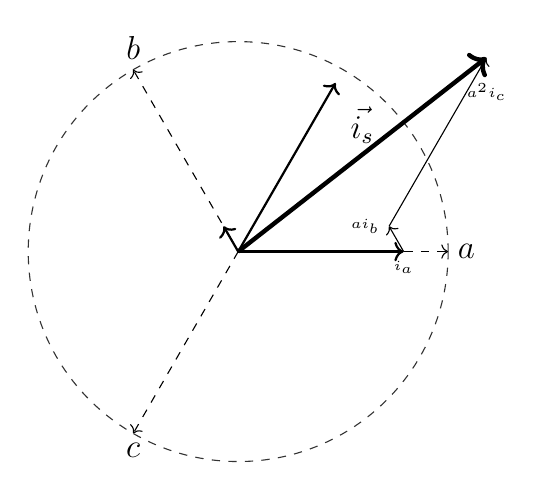
\begin{tikzpicture}
    \def \angle {38}
    %Definitions - These can be changed to create new figures%
    %===========================================================
    \def \Vs {4}; %Magnitude of space vector in cm
    \def \Angle {\angle}; %Angle with regards to phase A	
    %Calculated variables. These should not be changed unless you know what you are doing%
    %===========================================================
    \pgfmathsetmacro \Vmax {\Vs * 2/3}; %Max phase voltage
    \def \Axisheight {\Vmax *3};
    \pgfmathsetmacro \Va {\Vmax * cos{(\Angle+0)}}; %Magnitude of phase A at angle \Angle
    \pgfmathsetmacro \Vb {\Vmax * cos{(\Angle-120)}}; %Magnitude of phase B at angle \Angle
    \pgfmathsetmacro \Vc {\Vmax * cos{(\Angle-240)}}; %Magnitude of phase C at angle \Angle
    %Locations%
    %===========================================================
    \def \OrigoX {0 cm}; % If you want to move the circle relative to the wave forms (default -5cm)
    \def \OrigoY {0 cm};
    \coordinate (origo) at (\OrigoX,\OrigoY); %Center of top phasor diagram
    \coordinate (phase_a) at (0:\Va cm); %Tip of phase A
    \coordinate (phase_b) at (120:\Vb cm); %Tip of phase B
    \coordinate (phase_c) at (240:\Vc cm) ; %Tip of phase C
    %=============================================================================================================
    %Actual three phase phasors%
    %=============================================================================================================
    \node at (origo) [circle,dashed,draw=black!80, inner sep=0pt,minimum size=\Vmax*2 cm] {}; %Circle with radius 100%
    \draw[->,color=black,  thick] (origo)  -- ++(phase_a); %Phase A phasor
    \draw[->,color=black,  thick] (origo)  -- ++(phase_b); %Phase B phasor
    \draw[->,color=black,  thick] (origo)  -- ++(phase_c); %Phase C phasor
    %SPACE VECTOR %
    \draw[->,ultra thick,black] (origo) -- ++($(phase_a) + (phase_b) + (phase_c)$) coordinate(Vstip) node[anchor=north east, above, midway] {\large $\vec{i_s}$}; %Space vector resultant
    \pgfgetlastxy{\XCoord}{\YCoord}; % X and Y coordinates of Space vector tip
    %Find space vector angle
    \pgfmathanglebetweenpoints{\pgfpointanchor{origo}{center}}{\pgfpointanchor{Vstip}{center}}
    \let\PhaseBlack\pgfmathresult;
    %Phasor guide lines%
    \draw[->,color=black, dashed] (origo)  -- ++(0:\Vmax cm)  node[anchor=west] {\large $a$};
    \draw[->,color=black, dashed] (origo) -- ++(120:\Vmax cm) node[anchor=south] {\large $b$};
    \draw[->,color=black, dashed] (origo)  -- ++(240:\Vmax cm) node[anchor=north] {\large $c$};
    \draw[->,color=black, thin] (origo) ++(phase_a) node[anchor=west, below] {\tiny $i_a$} -> ++(phase_b) node[anchor=west, left] {\tiny $ai_b$}; %Resultant help lines
    \draw[->,color=black, thin] (origo) ++(phase_a) ++(phase_b) -> ++(phase_c) node[anchor=south east, below, yshift= -0.2cm] {\tiny $a^2i_c$}; 
    \end{tikzpicture}%
	\caption{\label{Sinhro_spacevect}Kompleksni vektor statorskega toka \cite{LaTex}}
\end{figure}
\subsubsection{Clarkina preslikava $(a,b,c)\rightarrow \alpha,\beta$}    
\begin{figure}[h]
	\centering
    \begin{tikzpicture}
    \def \angle {38}
    %Definitions - These can be changed to create new figures%
    %===========================================================
    \def \Vs {4}; %Magnitude of space vector in cm
    \def \Angle {\angle}; %Angle with regards to phase A
    %Calculated variables. These should not be changed unless you know what you are doing%
    %===========================================================
    \pgfmathsetmacro \Vmax {\Vs * 2/3}; %Max phase voltage
    \def \Axisheight {\Vmax *3};
    \pgfmathsetmacro \Va {\Vmax * cos{(\Angle+0)}}; %Magnitude of phase A at angle \Angle
    \pgfmathsetmacro \Vb {\Vmax * cos{(\Angle-120)}}; %Magnitude of phase B at angle \Angle
    \pgfmathsetmacro \Vc {\Vmax * cos{(\Angle-240)}}; %Magnitude of phase C at angle \Angle	
    %Locations%
    %===========================================================
    \def \OrigoX {0 cm}; % If you want to move the circle relative to the wave forms (default -5cm)
    \def \OrigoYb {0 cm};
    \coordinate (origob) at (\OrigoX,\OrigoYb); %Center of center phasor diagram
    \coordinate (phase_a) at (0:\Va cm); %Tip of phase A
    \coordinate (phase_b) at (120:\Vb cm); %Tip of phase B
    \coordinate (phase_c) at (240:\Vc cm) ; %Tip of phase C
    
    \draw[->,color=black, thin] (origob)  -- ++(0:\Vmax cm)  node[anchor=west, below left] { $a$};
    \draw[->,color=black, thin] (origob) -- ++(120:\Vmax cm) node[anchor=south] { $b$};
    \draw[->,color=black, thin] (origob)  -- ++(240:\Vmax cm) node[anchor=north] { $c$};

    %=============================================================================================================
    %Alpha and Beta Phasors
    %=============================================================================================================
    %SPACE VECTOR %
    \draw[->,ultra thick,black] (origob) -- ++($(phase_a) + (phase_b) + (phase_c)$) coordinate(Vstipb)node[anchor=north east, above, midway] {\large $\vec{i_s}$}; %Space vector resultant
    \pgfgetlastxy{\XCoordb}{\YCoordb}; % X and Y coordinates of Space vector tip
    %Find space vector angle
    \pgfmathanglebetweenpoints{\pgfpointanchor{origob}{center}}{\pgfpointanchor{Vstipb}{center}}
    \let\PhaseBlackb\pgfmathresult;
    %plave črtkane osi alfa,beta 
    \draw[->,color=black ,dashed] (\OrigoX,\OrigoYb) -- ++(90:1.2*\Vs cm) node[anchor=west] {$\beta$-os};
    \draw[->,color=black ,dashed] (\OrigoX,\OrigoYb)  -- ++(0:1.2*\Vs cm) node[anchor=west] {$\alpha$-os};
    \draw[-,color=gray, thin, dashed] (\OrigoX, \YCoordb) -> (Vstipb); %Alpha help Line
    \draw[-,color=gray, thin, dashed] (\XCoordb, \OrigoYb) -> (Vstipb); %Beta help Line
    \draw[->,color=black, very thick] (origob)  -- ++(0,\YCoordb-\OrigoYb) node[anchor=north east] {\large $i_{s\beta}$}; %Phase alpha phasor
    \draw[->,color=black, very thick] (origob)  -- ++(\XCoordb-\OrigoX,0) node[anchor=north] {\large $i_{s\alpha}$}; %Phase beta phasor
    \end{tikzpicture}%  
	\caption{\label{Sinhro_Clarke}Clarkina preslikava trifaznega sistema v $\alpha \beta$ koordinatni sistem}
\end{figure}   
Vektor statorskega toka se lahko zapiše kot vsoto realne in imaginarne komponente $\vec{i_s(t)}=i_{s\alpha}(t)+ji_{s\beta}(t)$, kar se po preobrazbi zapiše v enačbo \ref{Sinhr_ClarkeEn}
\begin{equation} \label{Sinhr_ClarkeEn}
\begin{aligned}
i_{s\alpha}(t) &= \dfrac{3}{2}i_{sa}(t)\\[5pt]
i_{s\beta}(t) &= \dfrac{\sqrt{3}}{2}\big(i_{sb}(t)-i_{sc}(t)\big)\\[5pt]
\end{aligned}
\end{equation}
Ob upoštevanju dejstva, da je $i_a+i_b+i_c=0$, se v praksi ne uporablja tri tokovne merilnike pač pa samo dva in se tok v tretji veji preračuna. Zato se enačbo \ref{Sinhr_ClarkeEn} zapiše v obliko, kjer se merita samo tokova $a$ in $b$:
\begin{equation} \label{Sinhr_ClarkeEn2}
\begin{aligned}
i_{s\alpha}(t) &= \dfrac{3}{2}i_{sa}(t)\\[5pt]
i_{s\beta}(t) &= \dfrac{\sqrt{3}}{2}\big(2i_{sb}(t)-i_{sa}(t)\big)\\[5pt]
\end{aligned}
\end{equation}
Clarkina preslikava, preslika trifazni sistem $abc$ v dvofaznega $\alpha \beta$.
\subsubsection{Parkova preslikava} 
\begin{figure}[h]
	\centering
	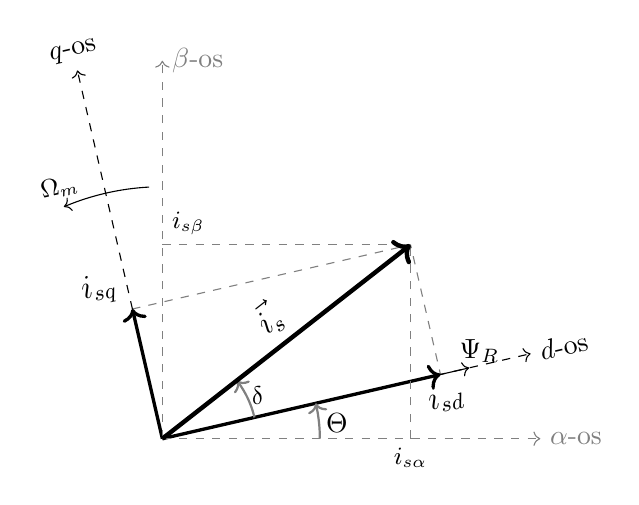
\begin{tikzpicture}
	\def \angle {38}
	%Definitions - These can be changed to create new figures%
	%===========================================================
	\def \Vs {4}; %Magnitude of space vector in cm
	\def \Angle {\angle}; %Angle with regards to phase A
	\def \Osv {25}; %Angle of d-axis wrt space vector
	\def \R {4}; %Magnitude of rotor flux in cm
	%Calculated variables. These should not be changed unless you know what you are doing%
	%===========================================================
	\pgfmathsetmacro \Qmag {\Vs * sin{\Osv})}; %Magnitude of Q axis
	\pgfmathsetmacro \Dmag {\Vs * cos{\Osv})}; %Magnitude of Q axis
	\pgfmathsetmacro \Vmax {\Vs * 2/3}; %Max phase voltage
	\pgfmathsetmacro \Va {\Vmax * cos{(\Angle+0)}}; %Magnitude of phase A at angle \Angle
	\pgfmathsetmacro \Vb {\Vmax * cos{(\Angle-120)}}; %Magnitude of phase B at angle \Angle
	\pgfmathsetmacro \Vc {\Vmax * cos{(\Angle-240)}}; %Magnitude of phase C at angle \Angle
	%Locations%
	%===========================================================
	\def \OrigoX {0cm}; % If you want to move the circle relative to the wave forms (default -5cm)
	\def \OrigoYc {0 cm};
	\coordinate (origoc) at (\OrigoX,\OrigoYc); %Center of bottom phasor diagram
	\coordinate (phase_a) at (0:\Va cm); %Tip of phase A
	\coordinate (phase_b) at (120:\Vb cm); %Tip of phase B
	\coordinate (phase_c) at (240:\Vc cm) ; %Tip of phase C
	%=============================================================================================================
	%%D and Q Phasors%
	%=============================================================================================================
	%Space Vector
	\coordinate (Vstipc) at  ($(origoc)+ (phase_a) + (phase_b) + (phase_c)$) ;
	
	\path (Vstipc);
	\pgfgetlastxy{\XCoordc}{\YCoordc}; % X and Y coordinates of Space vector tip
	%Find space vector angle
	\pgfmathanglebetweenpoints{\pgfpointanchor{origoc}{center}}{\pgfpointanchor{Vstipc}{center}}
	\let\PhaseBlackc\pgfmathresult;
	\coordinate (d1c) at (\PhaseBlackc-\Osv:1.2*\Vs cm) ; %Tip of d axis
	\coordinate (d2c) at (\PhaseBlackc-\Osv:-\Vs cm) ; %Tip of d axis
	\coordinate (q1c) at (\PhaseBlackc-\Osv+90:1.2*\Vs cm) ; %Tip of q axis
	\coordinate (q2c) at (\PhaseBlackc-\Osv+90:-\Vs cm) ; %Tip of q axis
	
	\coordinate (d3c) at (\PhaseBlackc-\Osv+90:\Qmag) ; %Tip of d 
	\coordinate (q3c) at (\PhaseBlackc-\Osv:\Dmag) ; %Tip of q 
	
	\draw[-,color=gray, thin, dashed] (origoc)  -- ++(d3c) -> (Vstipc); %Q help Line
	\draw[-,color=gray, thin, dashed] (origoc)  -- ++(q3c) -> (Vstipc); %Q help Line
	
	\draw[->,color=black, dashed] (origoc)  -- ++(d1c) node[rotate=\PhaseBlackc-\Osv,right] {$d$-os}; %D axis help line
	%    \draw[-,color=green, thin] (origoc)  -- ++(d2c); %D axis help line
	\draw[->,color=black, dashed] (origoc)  -- ++(q1c) node[rotate=\PhaseBlackc-\Osv, above] {$q$-os}; %Q axis help line
	%   \draw[-,color=green, thin] (origoc)  -- ++(q2c); %Q axis help line
	
	%% Rotor Flux Vector%
	\coordinate (rfluxtipc) at (\PhaseBlackc-\Osv:\R); %Tip of rotor flux
	\draw[->,color=black, thin] (origoc)  -- ++(rfluxtipc)  node[label={[label distance=-0.38cm]\PhaseBlackc-\Osv: $\Psi_R$}] {}; %Bottom Rotor Flux Phasor
	
	\draw[->,color=black, very thick] (origoc)  -- ++(d3c) node[rotate=\PhaseBlackc-\Osv, anchor=north east, above left] {\large $i_{sq}$}; %D phasor
	\draw[->,color=black, very thick] (origoc)  -- ++(q3c) node[rotate=\PhaseBlackc-\Osv, anchor=north] {\large $i_{sd}$}; %Q phasor
	
	% angular velocity \omega
	\draw[->] (\OrigoX,\OrigoYc) ++(\PhaseBlackc-\Osv+90-10:0.8*\Vs) arc (\PhaseBlackc-\Osv+90-10:\PhaseBlackc-\Osv+90+10:0.8*\Vs) node[rotate=\PhaseBlackc-\Osv,above]{\small $\Omega_{m}$};	
	% Angle between rotor and stator
	\draw[->, thick, color=gray] (\OrigoX,\OrigoYc) ++(\PhaseBlackc-\Osv:.3*\Vs) arc (\PhaseBlackc-\Osv:\PhaseBlackc:.3*\Vs) node[rotate=\PhaseBlackc-\Osv, below right,color=black] {\small $\delta$};	
	
	% kot rotorja glede na mirovno točko statorja
	%\draw[->, thick, color=violet] (\OrigoX,\OrigoYc) ++(\PhaseBlackc-\Osv:.5*\Vs) arc (\PhaseBlackc-\Osv:0:.5*\Vs) node[ below right,color=black] {$\Theta$};	
	\draw[->, thick, color=gray] (\OrigoX,\OrigoYc) ++(0:.5*\Vs) arc (0:\PhaseBlackc-\Osv:.5*\Vs) node[ below right,color=black] {$\Theta$};
	
	%plave črtkane osi alfa,beta
	\draw[->,color=gray ,dashed] (\OrigoX,\OrigoYc ) -- ++(90:1.2*\Vs cm) node[anchor=west] {$\beta$-os};
	\draw[->,color=gray ,dashed] (\OrigoX,\OrigoYc)  -- ++(0:1.2*\Vs cm) node[anchor=west] {$\alpha$-os};
	
	%alfa beta črtice
	\draw[-,color=gray, thin, dashed] (\OrigoX, \YCoordc) -- (Vstipc); %Alpha help Line
	\draw[-,color=gray, thin, dashed] (\XCoordc, \OrigoYc) -- (Vstipc); %Beta help Line
	\coordinate (origoc)  -- ++(0,\YCoordc-\OrigoYc) node[above right ] {\small $i_{s\beta}$}; %Phase alpha phasor
	\coordinate (origoc)  -- ++(\XCoordc-\OrigoX,0) node[below] {\small $i_{s\alpha}$}; %Phase beta phasor
	\draw[->,ultra thick,black] (origoc) -- ++($(phase_a) + (phase_b) + (phase_c)$) coordinate(Vstipc) node[rotate=\PhaseBlackc, anchor=north east, above, midway] {\large $\vec{i_s}$}; %Space vector resultant
	\end{tikzpicture}%
	\caption{\label{Sinhro_Park}Parkova preslikava  v $dq$ koordinatni sistem}
\end{figure} 
Parkova preslikava, preslika dvofazni sistem $\alpha \beta$ v rotirajoči koordinatni sistem $dq$. Pri sinhronskem motorju s trajnimi magneti je $d$-os fiksirana na rotor trajnega magneta in celotni koordinatni sistem sledi poziciji (kotu) rotorja $\Theta$. V ta namen je uporabljen absolutni dajalnik pozicije.\\
\begin{equation} \label{Sinhr_ParkEn}
\begin{aligned}
i_{sd}(t) &= i_{s\alpha}(t)cos(\Theta)+i_{s\beta}(t)sin(\Theta)\\[5pt]
i_{sq}(t) &= -i_{s\alpha}(t)sin(\Theta)+i_{s\beta}(t)cos(\Theta)\\[5pt]
\end{aligned}
\end{equation}
Enačba \ref{Sinhr_ParkEn} opisuje Parkovo preslikavo v $dq$ rotirajoči koordinatni sistem Uporabno dejstvo te pretvorbe je to, da sedaj posamezne komponente predstavljao vzbujanje $d$ in navor $q$, podobno kot pre enosmernem tuje vzbujanem motorju. V ustalejnem stanju sta ti dve komponenti časovno nespremenljive, čeprav se motor vrti s polno hitrostjo.
Na sliki \ref{Sinhro_Park} je prikazan tak rotirajoči kazalčni diagram, pri čemer so veliosti komponent $i_{sd}$ in $i_{sq}$ izbrane za lepši pregled diagrama, ne predstavljajo pa stanja v realnem, pravilno izkrmiljenem motorju. Rotorski fluks $\Psi_R$ je rezultat delovanja trajnega magneta, ne pa posledica vpliva statorskih veličin na rotor. Enačba za navor sinhronskega motorja je \cite{ambrovzivc1996sodobne}:
\begin{equation} \label{Sinhr_moment}
M_{el} = \Psi_Ri_{sq}\\[5pt]
\end{equation}
Največji navor dobimo takrat, ko ima celoten statorski tok le $q$ komponento, se pravi $i_{sd}=0$.
\subsubsection{Inverzna Parkova in Clarkina preslikava}
Iz želenih vrednosti $i^*_{sd}$ in $i^*_{sq}$ in njihove povratne informacije se z uporabo PI regulatorja pridobi vrednosti želenih statorskih napetosti $u^*_{sd}$ in $u^*_{sq}$ in se jih preslika v $\alpha \beta$ koordinatni sistem s pomočjo inverzne Parkove preslikave (enačba \ref{Sinhr_InvParkEn}) \cite{instruments1998field}.
\begin{equation} \label{Sinhr_InvParkEn}
\begin{aligned}
u^*_{\alpha}(t) &= u^*_{sd}(t)cos(\Theta)-u^*_{sq}(t)sin(\Theta)\\[5pt]
u^*_{\beta}(t) &= u^*_{sd}(t)sin(\Theta)+u^*_{sq}(t)cos(\Theta)\\[5pt]
\end{aligned}
\end{equation}
Kazalčni diagram \ref{Sinhro_InvPark} prikazuje vektor statorske napetosti ter vektor statorskega  toka. Pri sinhroskem motorju s trajnim magnetom je zaželno, da je $i_{sd}=0$, ali pa celo negativen v kolikor se želi obratovati v področju slabljenja polja. Za doseganje višjega števila obratov od nazivnih se z negativnim tokom $i_{sd}$ doseže zmanjšan rotorski fluks $\Psi_R$, zaradi nasprotnega delovanja statorskega fluksa v d-osi. Tak način obratovanja je za sinhronski motor s trajnimi magneti zelo redek.\\
Asinhronski motorji se tudi lahko krmilijo na način orientacije polja, vendar je tedaj vzbujalna komponenta $i_{sd}$ prisotna. Ker se rotorski fluks ne giblje z isto krožno frekvenco kot statorski, temveč zaostaja s frekvenco slipa, je potrebna drugačna, bolj kompleksna metoda za izračun rotorskega vektroja fluksa.  
\begin{figure}[h]
	\centering
	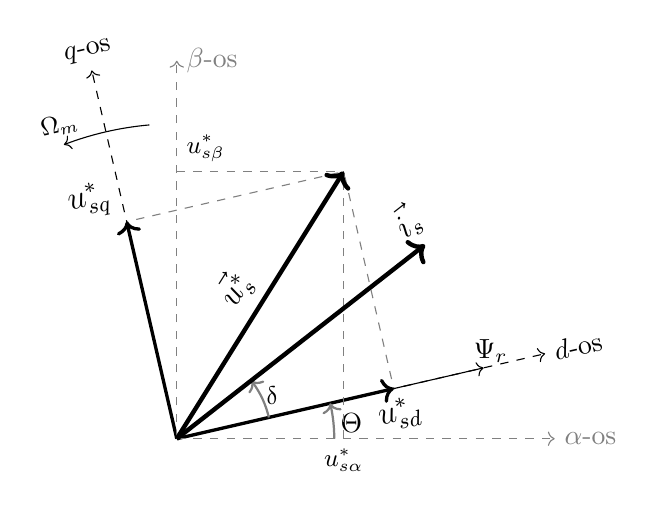
\begin{tikzpicture}
	\def \angle {38}
	\def \Osv {25}; %Angle of d-axis wrt space vector
	\def \NapZamik {20}; %zamik napetosti napram statorskemu toku
	%Definitions - These can be changed to create new figures%
	%===========================================================
	\def \Vs {4}; %Magnitude of space vector in cm
	\def \Angle {\angle}; %Angle with regards to phase A
	
	\def \R {4}; %Magnitude of rotor flux in cm
	%Calculated variables. These should not be changed unless you know what you are doing%
	%===========================================================
	\pgfmathsetmacro \Qmag {\Vs * sin{(\Osv+\NapZamik)}}; %Magnitude of Q axis
	\pgfmathsetmacro \Dmag {\Vs * cos{(\Osv+\NapZamik})}; %Magnitude of Q axis
	\pgfmathsetmacro \Vmax {\Vs * 2/3}; %Max phase voltage
	\pgfmathsetmacro \Va {\Vmax * cos{(\Angle+0)}}; %Magnitude of phase A at angle \Angle
	\pgfmathsetmacro \Vb {\Vmax * cos{(\Angle-120)}}; %Magnitude of phase B at angle \Angle
	\pgfmathsetmacro \Vc {\Vmax * cos{(\Angle-240)}}; %Magnitude of phase C at angle \Angle
	%Locations%
	%===========================================================
	\def \OrigoX {0cm}; % If you want to move the circle relative to the wave forms (default -5cm)
	\def \OrigoYc {0 cm};
	\coordinate (origoc) at (\OrigoX,\OrigoYc); %Center of bottom phasor diagram
	\coordinate (phase_a) at (0:\Va cm); %Tip of phase A
	\coordinate (phase_b) at (120:\Vb cm); %Tip of phase B
	\coordinate (phase_c) at (240:\Vc cm) ; %Tip of phase C
	%=============================================================================================================
	%%D and Q Phasors%
	%=============================================================================================================
	%Space Vector
	\coordinate (Vstipc) at  ($(origoc)+ (phase_a) + (phase_b) + (phase_c)$) ;
	
	\path (Vstipc);
	\pgfgetlastxy{\XCoordc}{\YCoordc}; % X and Y coordinates of Space vector tip
	%Find space vector angle
	\pgfmathanglebetweenpoints{\pgfpointanchor{origoc}{center}}{\pgfpointanchor{Vstipc}{center}}
	\let\PhaseBlackc\pgfmathresult;
	
	\coordinate (dVs) at (\PhaseBlackc+\NapZamik: \Vs cm) ; %Tip Vs
	\path (dVs);
	\pgfgetlastxy{\XCoordc}{\YCoordc}; % X and Y coordinates of Space vector tip
	
	\coordinate (d1c) at (\PhaseBlackc-\Osv:1.2*\Vs cm) ; %Tip of d axis
	\coordinate (d2c) at (\PhaseBlackc-\Osv:-\Vs cm) ; %Tip of d axis
	\coordinate (q1c) at (\PhaseBlackc-\Osv+90:1.2*\Vs cm) ; %Tip of q axis
	\coordinate (q2c) at (\PhaseBlackc-\Osv+90:-\Vs cm) ; %Tip of q axis
	
	\coordinate (d3c) at (\PhaseBlackc-\Osv+90:\Qmag) ; %Tip of d 
	\coordinate (q3c) at (\PhaseBlackc-\Osv:\Dmag) ; %Tip of q 
	\draw[-,color=gray, thin, dashed] (origoc)  -- ++(d3c) -> (dVs); %Q help Line
	\draw[-,color=gray, thin, dashed] (origoc)  -- ++(q3c) -> (dVs); %Q help Line
	
	\draw[->,color=black, dashed] (origoc)  -- ++(d1c) node[rotate=\PhaseBlackc-\Osv,right] {$d$-os}; %D axis help line
	%    \draw[-,color=green, thin] (origoc)  -- ++(d2c); %D axis help line
	\draw[->,color=black, dashed] (origoc)  -- ++(q1c) node[rotate=\PhaseBlackc-\Osv, above] {$q$-os}; %Q axis help line
	%   \draw[-,color=green, thin] (origoc)  -- ++(q2c); %Q axis help line
	
	%% Rotor Flux Vector%
	\coordinate (rfluxtipc) at (\PhaseBlackc-\Osv:\R); %Tip of rotor flux
	\draw[->,color=black, thin] (origoc)  -- ++(rfluxtipc)  node[label={[label distance=-0.38cm]\PhaseBlackc-\Osv: $\Psi_r$}] {}; %Bottom Rotor Flux Phasor
	
	\draw[->,color=black, very thick] (origoc)  -- ++(d3c) node[rotate=\PhaseBlackc-\Osv, anchor=north east, above left] {\large $u^*_{sq}$}; %D phasor
	\draw[->,color=black, very thick] (origoc)  -- ++(q3c) node[rotate=\PhaseBlackc-\Osv, anchor=north] {\large $u^*_{sd}$}; %Q phasor
	
	% angular velocity \omega
	\draw[->] (\OrigoX,\OrigoYc) ++(\PhaseBlackc-\Osv+90-8:1*\Vs) arc (\PhaseBlackc-\Osv+90-8:\PhaseBlackc-\Osv+90+8:1*\Vs) node[rotate=\PhaseBlackc-\Osv,above]{\small $\Omega_{m}$};	
	% Angle between rotor and stator
	\draw[->, thick, color=gray] (\OrigoX,\OrigoYc) ++(\PhaseBlackc-\Osv:.3*\Vs) arc (\PhaseBlackc-\Osv:\PhaseBlackc:.3*\Vs) node[rotate=\PhaseBlackc-\Osv, below right,color=black] {\small $\delta$};	
	
	% kot rotorja glede na mirovno točko statorja
	%\draw[->, thick, color=violet] (\OrigoX,\OrigoYc) ++(\PhaseBlackc-\Osv:.5*\Vs) arc (\PhaseBlackc-\Osv:0:.5*\Vs) node[ below right,color=black] {$\Theta$};	
	\draw[->, thick, color=gray] (\OrigoX,\OrigoYc) ++(0:.5*\Vs) arc (0:\PhaseBlackc-\Osv:.5*\Vs) node[ below right,color=black] {$\Theta$};
	
	%plave črtkane osi alfa,beta
	\draw[->,color=gray ,dashed] (\OrigoX,\OrigoYc ) -- ++(90:1.2*\Vs cm) node[anchor=west] {$\beta$-os};
	\draw[->,color=gray ,dashed] (\OrigoX,\OrigoYc)  -- ++(0:1.2*\Vs cm) node[anchor=west] {$\alpha$-os};
	
	%alfa beta črtice
	\draw[-,color=gray, thin, dashed] (\OrigoX, \YCoordc) -- (dVs); %Alpha help Line
	\draw[-,color=gray, thin, dashed] (\XCoordc, \OrigoYc) -- (dVs); %Beta help Line
	\coordinate (origoc)  -- ++(0,\YCoordc-\OrigoYc) node[above right ] {\small $u^*_{s\beta}$}; %Phase alpha phasor
	\coordinate (origoc)  -- ++(\XCoordc-\OrigoX,0) node[below] {\small $u^*_{s\alpha}$}; %Phase beta phasor
	\draw[->,ultra thick,black] (origoc) -- ++($(phase_a) + (phase_b) + (phase_c)$) coordinate(Vstipc) node[rotate=\PhaseBlackc, anchor=north east, above] {\large $\vec{i_s}$}; %Space vector resultant
	
	\draw[->,ultra thick,black] (origoc) -- ++(\PhaseBlackc +\NapZamik:\Vs cm) node[rotate=\PhaseBlackc+\NapZamik, anchor=north east, above, midway] {\large $\vec{u^*_s}$}; %Space vector resultant
	\end{tikzpicture}%
\caption{\label{Sinhro_InvPark} Inverzna Parkova preslikava iz $dq$ v $\alpha \beta$ koordinatni sistem}
\end{figure} 	
Inverzna Clarkina transformacije je izvedena direktno z modulacijo presmerniškega mostiča. Najbolj pogosta oblika modulacije se imenuje prostorka pulzno-širinska modulacija (angl. Space Vector Pulse Width Modulation - SVPWM).
\section{Asinhronski motor}
\begin{figure}[h]
	\centering
	\includegraphics[width=0.7\columnwidth]{Asinhronc.jpg}
	\caption{\label{Asinh_slika}Prečni prerez asinhornskega motorja s kratkostično kletko}
\end{figure}
\begin{circuitikz}[american voltages, european inductors]
	\draw
	% rotor circuit
	(0,0) to [short, *-] (6,0)
	to [V, l_=$\vec{U_i}$] (6,2) % rotor emf
	to [R, l_=$R_R$] (6,4) % rotor resistance
	to [short, i_=$\vec{I}_R$] (5,4) % rotor current
	
	% stator circuit
	(0,0) to [open, v^>=$\vec{U}_s$] (0,4) % stator voltage
	to [short, *- ,i=$\vec{I}_s$] (1,4) % stator current
	to [R, l=$R_s$] (3,4) % stator resistance
	to [L, l=$L_{\sigma}$] (5,4) % leakage inductance
	to [short, i_=$\vec{I}_m$] (5,3) % magnetizing current
	to [L, l_=$L_M$] (5,0); % magnetizing inductance
\end{circuitikz}
\subsubsection{Krmiljenje z U/f karakteristiko }
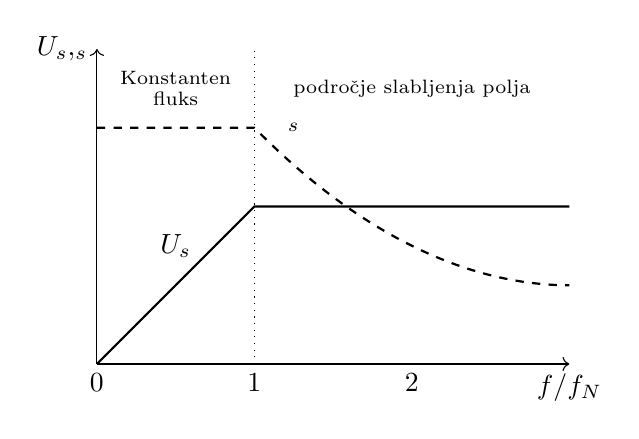
\begin{tikzpicture}
% horizontal axis
\draw[->] (0,0) -- (6,0) node[anchor=north] {$f/f_N$};
% labels
\draw	(0,0) node[anchor=north] {0}
(2,0) node[anchor=north] {1}
(4,0) node[anchor=north] {2};
% ranges
\draw	(1,3.5) node[align=center]{\shortstack{\scriptsize Konstanten\\\scriptsize fluks}}
(4,3.5) node{{\scriptsize področje slabljenja polja}};
% vertical axis
\draw[->] (0,0) -- (0,4) node[anchor=east] {$U_s,\varPsi_s$};
% nominal speed
\draw[dotted] (2,0) -- (2,4);
% Us
\draw[thick] (0,0) -- (2,2) -- (6,2);
\draw (1,1.5) node {$U_s$}; %label
% Psis
\draw[thick,dashed] (0,3) -- (2,3) parabola[bend at end] (6,1);
\draw (2.5,3) node {$\varPsi_s$}; %label
\end{tikzpicture}
\subsubsection{Vektroski način krmiljenja}
\subsubsection{Tehnika 87Hz}
\subsubsection{Pogoste težave frekvenčnih pretvornikov}
\begin{figure}[h]
		\centering
		\resizebox{0.5\textwidth}{!}{%
	\begin{circuitikz}[european inductors, scale=2]
		\def\xPortLeft{0}
		\def\xC{1.5}
		\def\xPortRight{3}	
		\def\yTerminalBottom{1}
		\def\yBottomGND{0}
		\def\yUpperGND{4}		
		\def\yL{2}
		\def\yR{1.5}
		\def\yC{3}	
		\draw                               (\xPortLeft,\yC)
		to[short,i=$i_{inv}$]                   (\xC,\yC)
		to[C, i>^= $C\frac{du}{dt}$ , l_=$C_{ff}$,*-*]           (\xC,\yTerminalBottom)
		to[short]          (\xPortLeft,\yTerminalBottom)
		to[open,v^<=$u_{inv}$,o-o]   (\xPortLeft,\yC);
		
		\draw                               (\xC,\yC)
		to[short, i=$i_S$]                   (\xPortRight,\yC)
		to[L=$L_S$]               (\xPortRight, \yL)
		to[R=$R_S$]                   (\xPortRight, \yR)
		to[short]                   (\xPortRight,\yTerminalBottom)
		to[short]                   (\xC,\yTerminalBottom);
		
		\draw                               (\xC,\yC)
		to[C, l_=$C_{fz}$]           (\xC,\yUpperGND) node[ground, rotate= 180]{} ;
		\draw                               (\xC,\yTerminalBottom)
		to[C, l_=$C_{fz}$]           (\xC,\yBottomGND) node[ground]{};
	\end{circuitikz}}
	\caption{\label{Asinhron_parazit}Tokovni pulzi zaradi parazitne kapacitivnosti kabla}
\end{figure}

\begin{figure}[h]
	\begin{circuitikz}[european inductors]
		\def\xPortLeft{0}
		\def\xPortRight{6}	
		\def\xL{1}	
		\def\xLend{2}
		\def\yTerminalBottom{1}
		\def\yLa{1.6}
		\def\yLb{0.8}
		\def\yLc{0}	
		\def\yLac{2}
		\def\yLbc{1.2}
		\def\yLcc{0.4}	
		\def\xLcrt{2.2}	
		
		\draw                               (\xPortLeft, \yLa)
		to[short, o-]         	(\xL,\yLa)
		to[L]           	     (\xLend,\yLa)
		to[short, i=$i_{S_U}$]            	(\xPortRight,\yLa);
		\draw[dashed] (\xL,\yLac) -- (\xLcrt,\yLac);
		
		\draw                               (\xPortLeft, \yLb)
		to[short, o-]                   (\xL,\yLb)
		to[L]           (\xLend,\yLb)
		to[short, i=$i_{S_V}$]            	(\xPortRight,\yLb);
		\draw[dashed] (\xL,\yLbc) -- (\xLcrt,\yLbc);
		
		\draw                               (\xPortLeft, \yLc)
		to[short, o-]                   (\xL,\yLc)
		to[L]           (\xLend,\yLc)
		to[short, i=$i_{S_W}$]            	(\xPortRight,\yLc);
		\draw[dashed] (\xL,\yLcc) -- (\xLcrt,\yLcc);
		
		\draw[dashed] (\xLcrt,\yLac) -- (\xLcrt,\yLcc);
		\draw [black,fill=white] (\xPortRight,\yLb) circle [radius=1cm] node{M}; 
	\end{circuitikz}
	\caption{\label{Asinhron_reaktor}Dušilka na izhodu iz frekvenčnega pretvornika}
\end{figure}
\chapter{Mehanska prilagoditev stroja}
Električni stroj žene breme, ki ima svoj vztrajnostni moment in deluje z določeno nazivno hitrostjo, zato je potrebno prilagoditi hitrost motorja bremenu. Na splošno uprabljeni elementi strojništva za ta namene so planetni reduktorji, zobniški prenosi, jermenice,...itd. Za optimalno delovanje celotnega sklopa je priporočljivo, da je preslikan bremenski vztrajnostni moment enak vztrajnostnem momentu rotorja motorja. Le tako se lahko doseže najboljši odziv regulacijskega kroga. Na sliki \ref{Mehanika_reduktor} je prikazan princip mehanskega reduktorja s prestavnin razmerjem $p$. Izhodna hitrost iz reduktorja je tako: $\Omega_L = \dfrac{\Omega_R}{p}$, navor pa $M_L=M\cdot p$. Skoraj najpomemnejši podatek pa je preslikan vztrajnostni moment na vhodno stran reduktorja: $J_L'=\dfrac{J_L}{p^2}$, ki skupaj z vtrajnostnim momentom rotorja predstavlja vtrajnostni moment sistema: $J_S=J_R+J_L'$. Pomembna lastnost sklopa je ta, da izhodna hitrost upada sorazmerno s prestavnim razmerjem, preslikan vztrajnostni moment pa kvadratično, kar je zelo ugodno pri izbiri ustreznega prestavnega razmerja in tipa motorja.\\
\begin{figure}[h]
	\centering
	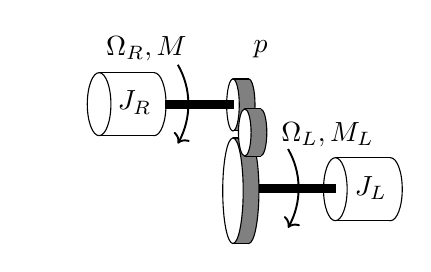
\begin{tikzpicture}
	%	\draw [help lines] (-1,-2) grid (12,5);	
	% moment of inertia
	\draw[fill=white] (5.5,1.5) ellipse (.15 and 0.4);
	\draw[fill=white, color=white] (3.9, 1.9) rectangle (5.49, 1.1);
	\draw (4.8,1.5) ellipse (.15 and 0.4);
	\draw (4.8,1.9) -- (5.5,1.9);
	\draw (4.8,1.1) -- (5.5,1.1);		
	\draw (5.25,1.52) node {$J_R$};
	
	% transmission gear one
	\draw[fill=black!50] (6.7,1.49)
	ellipse (.08 and 0.33);
	\draw[fill=black!50, color=black!50] (6.7,1.82)
	rectangle (6.5,1.16);
	\draw[fill=white] (6.5,1.49)
	ellipse (.08 and 0.33);
	\draw (6.5,1.82) -- (6.7,1.82);
	\draw (6.5,1.16) -- (6.7,1.16);
	
	% shaft drive -> transmission
	\draw[fill=black] (5.65,1.45) rectangle (6.5,1.55);
	
	% momentum arrow of drive -> transmission
	\draw[line width=0.7pt,<-] (5.8,1) arc (-30:30:1);
	
	% transmission gear two
	\draw[fill=black!50] (6.7,0.40)
	ellipse (.13 and 0.67);
	\draw[fill=black!50, color=black!50] (6.7,1.07)
	rectangle (6.5,-0.27);
	\draw[fill=white] (6.5,0.40)
	ellipse (.13 and 0.67);
	\draw (6.5,1.07) -- (6.7,1.07);
	\draw (6.5,-0.27) -- (6.7,-0.27);
	
	% transmission gear three
	\draw[fill=black!50] (6.85,1.14)
	ellipse (.08 and 0.3);
	\draw[fill=black!50, color=black!50] (6.85,1.44)
	rectangle (6.65,0.84);
	\draw[fill=white] (6.65,1.14)
	ellipse (.08 and 0.3);
	\draw (6.65,1.44) -- (6.86,1.44);
	\draw (6.65,0.84) -- (6.86,0.84);
	
	% transmission shaft from gear two to moment of inertia
	\draw[fill=black] (6.84,0.38) rectangle (7.8,0.48);
	
	% moment of inertia
	\draw[fill=white] (8.5,0.42)
	ellipse (.15 and 0.4);
	\draw[fill=white, color=white] (7.9, 0.82)
	rectangle (8.49, 0.02);
	\draw (7.8,0.42) ellipse (.15 and 0.4);
	\draw (7.8,0.82) -- (8.5,0.82);
	\draw (7.8,0.02) -- (8.5,0.02);
	% momentum arrow between transmission and moment of inertia
	\draw[line width=0.7pt,<-] (7.2,-0.07) arc (-30:30:1);
	% descriptions inside graphic
	\draw (5.4,2.2) node {$\Omega_R, M$};
	\draw (7.7,1.11) node {$\Omega_L, M_L$};
	\draw (8.25,0.44) node {$J_L$};
	\draw (6.85,2.2) node {$p$};
	\end{tikzpicture}
	\caption{\label{Mehanika_reduktor}Mehanski reduktor}
\end{figure}

Najprej je potrebno določiti vztrajnostni moment bremena ter hitrosti pomikov, nato se iz proizvajalčevega kataloga servo motorjev izbere določen nabor motorjev s podatki o vztrajnostnem momentu motorja in nominalno hitrostjo. Naparavi se tabela izračunov preslikave vztrajnostnega momneta bremena v odvisnosti od prestavnega razmerja in nato primerja z vztrajnostnim momentom rotorja in tako izbere ustrezen tip motorja. Proizvajalci imajo običajno nabor sinhronskih servo motorjev z različnimi vztrajnostnimi momenti pri skoraj enaki izhodni moči motorja. Imenovani so angl. high inertia, standard, high dynamics; to so motorji z velikim, standardnim ali majhnim vztrajnostnim momentom. Za izjemno dinamične sisteme pa obstajajo še prisilno hlajeni servo motorji, zračno ali vodno. Standardni motorji so konvekcijsko hlajeni, večje kot nazivne moči, so tudi motorji večjih dimenzij in s tem imajo tudi večji vztrajnostni moment. Posebna oblika visoko dinamičnih motorjev je ta, da se za večjo moč motorja ne uporabi večanje dimenzij ampak tokovno obrementitev in zato postane potreba po prisilnem hlajenju. Motorji z naječjo dinamiko so tako vodno hlajeni, kar pomeni zajeten strošek saj potrebuje zraven še hladilni sistem.\\   
Pri sami oblike montaže motorja na reduktor je potrebno še posebna pozornost, namreč spojka katera objema rotorsko gred ima lahko velik vtrajnostni moment v primerjavi z rotorjem, tu gre seveda za motorje z visoko dinamiko. Pri izbiri motorja z visoko dinamiko, prav vsi dodatki kot so dajalnik pozicije in elektromehanska zavora, znatno prispevajo h končnem vztrajnostnem mommentu sistema, saj ostale vrteče se mase na izhodu reduktorja nimajo takšen velik vpliv. 
\subsection{Mehanska resonanca in anti-resonanca}
\begin{figure}[h]
	\centering
	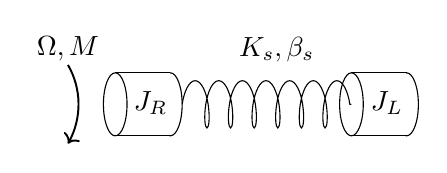
\begin{tikzpicture}
	%	\draw [help lines] (-1,-2) grid (12,5);
	% moment of inertia
	\draw[fill=white] (5.5,1.5) ellipse (.15 and 0.4);
	\draw[fill=white, color=white] (3.9, 1.9) rectangle (5.49, 1.1);
	\draw (4.8,1.5) ellipse (.15 and 0.4);
	\draw (4.8,1.9) -- (5.5,1.9);
	\draw (4.8,1.1) -- (5.5,1.1);		
	\draw (5.25,1.52) node {$J_R$};
	% moment of inertia
	\draw[fill=white] (8.5,1.5) ellipse (.15 and 0.4);
	\draw[fill=white, color=white] (6.9, 1.9) rectangle (8.49, 1.1);
	\draw (7.8,1.5) ellipse (.15 and 0.4);
	\draw (7.8,1.9) -- (8.5,1.9);
	\draw (7.8,1.1) -- (8.5,1.1);		
	\draw (8.25,1.52) node {$J_L$};
	\draw[decoration={aspect=0.3, segment length=3mm, amplitude=3mm,coil},decorate] (5.65,1.5) -- (7.8,1.5); 
	% momentum arrow of drive -> transmission
	\draw[line width=0.7pt,<-] (4.2,1) arc (-30:30:1);
	% descriptions inside graphic
	\draw (4.2,2.2) node {$\Omega, M$};
	%		\draw (7.29,1.11) node {$\omega_L$};
	%		\draw (8.25,0.44) node {$J_L$};
	\draw (6.85,2.2) node {$K_s,  \beta_s$};
	\end{tikzpicture} \caption{\label{Meh_Resonannca}Sklopljen sistem dveh vztrajnostnih mas}
\end{figure}
V realnosti ne obstaja možnost, da je breme togo sklopljeno z motorjem, ker ima vsaka osovina, jermen, zobnik,...ki povezuje os rotorja motorja z bremenom svojo elastičnost, in dušenje. Na sliki \ref{Meh_Resonannca} je prikaz sklopljenega sistema: rotor in breme sta povezana z osovino, katera ima koeficient torzije $K_s$ ter faktor dušenja $\beta_s$. Enačba \ref{Meh_trfcn} je prenosna funkcija hitrosti motorja v odvisnosti od izhodnega navora v Laplace-ovim prostoru \cite{yumrukccal2013dynamic}. Takšen sklopljen sistem dveh vztrajnostnih mas ima resonnančno $\omega_{res}$ in anti-resonančno $\omega_{Ares}$ krožno frekvenco nihanja (enačba \ref{Meh_res}) \cite{DesignTrends}.
\begin{equation} \label{Meh_trfcn}
\dfrac{\Omega(s)}{M(s)} = \dfrac{s^2J_L+s\beta_s+K_s}{s(J_L+J_R)(s^2\dfrac{(J_R+J_L)}{J_R\;J_L}+s\beta_s+K_s)}\\[5pt]
\end{equation}
\begin{equation} \label{Meh_res}
\begin{aligned}
\omega_{res} &= \sqrt{\dfrac{(J_R+J_L)\;K_s}{J_R\;J_L}}\\[5pt]
\omega_{Ares} &= \sqrt{\dfrac{K_s}{J_L}}\\[5pt]
\end{aligned}
\end{equation}
Anti-resonanca pomeni, da ob morebinem nihanju rotorja s to frekvenco, breme ostane v mirovanju. Tak sklop je na primer dvomasni vztrajnik v avtomobilu, ki preprečuje prenos vibracij motorja na menjalnik, vendar pri elektromotornih pogonih ta pojav nima bistvene teže. Veliko bolj problematičen je pojav resonance. Na splošno je želja, da bi mehanski sistem imel čim višjo resonančno frekvenco, ker je s tem povezan tudi dinamični odziv regulacijskega kroga. Za veliko dinamiko sistema je potrebno zagotoviti čim višje krožno ojačanje regulacijskega kroga in se tako pojavi težava osciliranja pri mehanski resonančni frekvenci. To se lahko deloma odpravi z dodajanjem korekcijskih členov v regulacijski krog, kateri izločijo določene frekvence. To so pasovno-zaporna frekvenčna sita, ki se jih vključi v regulacijski krog potem, ko se z eno od metod frekvenčne analize sistema določi resonančne frekvence, teh je običajno več, odvisno koliko kompleksen je sklop naprave.  
\chapter{Teorija regulacij in krmiljenja}
V primeru, da poznamo osnovno matematično relacijo med vhodom in izhodom nekega
sistema, bi lahko vnaprej določili vrednost vzbujanja, katerega bi vnesli v sistem, da bi dobili želeno izhodno vrednost iz sistema. Tak način vodenja imenujemo krmiljenje (slika \ref{Regulacije_Krmiljenje}), njegova značilnost je ta, da nima povratne zanke.\\
\begin{figure}[h]
	\begin{tikzpicture}[auto, node distance=2cm,>=latex']
	\node [input, name=input] {};
	\node [block, right of=input,  node distance=2cm] (krm) {Krmilnik};
	\node [block, right of=krm,  node distance=3cm] (sis) {Sistem};
	\node [output, right of=sis,  node distance=3cm] (out) {};
	\draw [draw,->] (input) -- node(a)[at start] {$y^*(t)$} (krm);	
	\draw [draw,->] (krm) -- node(b)[midway ] {$U(t)$} (sis);	
	\draw [draw,->] (sis) -- node(c)[at end ] {$W(t)$} (out);
	\node [name=a1, above of=a,  node distance=1.5cm, align=center]  {Želena/referenčna\\vrednost};
	\draw [->] (a1) --  (a);	
	\node [name=b1, above of=b,  node distance=1.5cm, align=center]  {Krmilna količina};
	\draw [->] (b1) --  (b);
	\node [name=c1, above of=c,  node distance=1.5cm, align=center]  {Krmiljena količina};
	\draw [->] (c1) --  (c);		
	\end{tikzpicture}	\caption{\label{Regulacije_Krmiljenje}Krmilni sistem}
\end{figure}

Slabost krmiljenja je občutljivost na zunanje vplive zaradi katerih pride do odstopanja med želeno in dejansko vrednostjo krmiljene količine. Kot ustrezna rešitev problema so so se pojavili regulirani sistemi, kjer merimo izhodno količino in jo nato primerjamo z želeno vrednostjo, tako dobimo pogrešek $\varepsilon$. Regulator nato nastavlja vhodno količino sistema in s tem poskrbi, da je pogrešek čim manjši oz. da se ta celo popolnoma odpravi \cite{pribec2014optimizacija}. 

\begin{figure}[h]
	\begin{tikzpicture}[auto, node distance=2cm,>=latex']
	\node [input, name=input] {};
	\node [sum, right of=input,  node distance=1.5cm] (eps) {};	
	\node [block, right of=eps,  node distance=3cm] (krm) {Regulator};
	\node [block, right of=krm,  node distance=3cm] (sis) {Sistem};
	\node [output, right of=sis,  node distance=3cm] (out) {};
	\draw [draw,->] (input) -- node(a)[at start] {$y^*(t)$} node[pos=0.95] {$+$}(eps);	
	\draw [draw,->] (eps) -- node(d)[midway ] {$\varepsilon (t)$} (krm);	
	\draw [draw,->] (krm) -- node(b)[midway ] {$u(t)$} (sis);	
	\draw [draw,->] (sis) -- node(e)[near start]{} node(c)[at end] {$w(t)$} (out);
	\node [name=a1, above of=a,  node distance=1.5cm, align=center]  {Želena/referenčna\\vrednost};
	\draw [->] (a1) --  (a);	
	\node [name=b1, above of=b,  node distance=1.5cm, align=center]  {Regulirna količina};
	\draw [->] (b1) --  (b);
	\node [name=c1, above of=c,  node distance=1.5cm, align=center]  {Regulirana količina};
	\draw [->] (c1) --  (c);		
	\node [name=d1, above of=d,  node distance=1.5cm, align=center]  {Pogrešek};
	\draw [->] (d1) --  (d);
	\draw[->] (e) |- ([yshift=-2cm]krm.south)-| node[above,near start]{povratna zanka} node[pos=0.95](){$-$}  (eps);   % tokovna povratna zanka
	
	\end{tikzpicture}	\caption{\label{Regulacije_Zaprt}Reguliran/zaprtozančni sistem}
\end{figure}

Regulirani sistemi (slika \ref{Regulacije_Zaprt}) imajo sklenjeno povratno zanko, zato te imenujemo
tudi zaprtozačne sisteme, krmiljene sistema pa odprtozančne. Ker noben fizikalen sistem ne deluje neskončno hitro, tudi od regulatorja ne moremo pričakovati, da bo trenutno opdravil spremembo, za to je potreben nek regulacijski čas. Regulacije delimo na linearne in nelinearne, odvisno od  členov, ki nastopajo v regulacijskem krogu. V linearnih regulacijah nastopajo le linearni členi. Če v regulacijskem krogu nastopa le en nelinearen člen, je regulacija nelinarna. Realen sistem je skoraj vedno nelinearen, večinoma je njegova statična karakteristika nelinearna, zato se ga linearizira v točki delovanja in se smatra, da je za majhne odmike sistem linearen in se ga opiše z diferencialnimi enačbami za dano dolovno točko \cite{Cajhen1990regulacije}.\\ 
\begin{figure}[h]
	\centering
	\resizebox{0.5\textwidth}{!}{%
	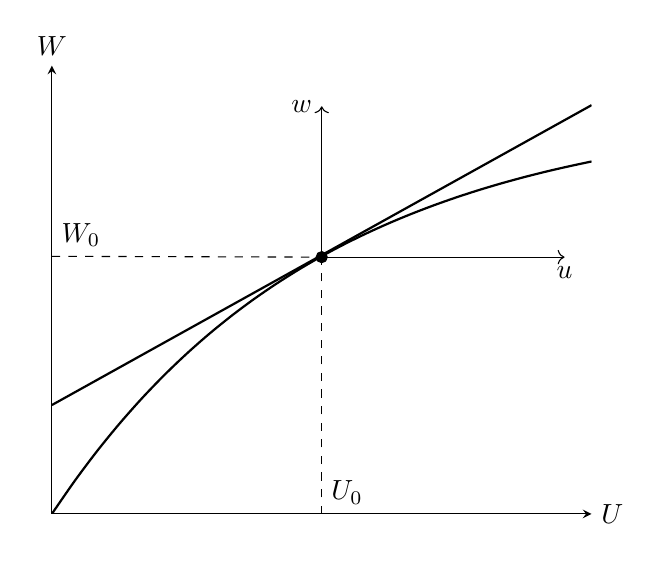
\begin{tikzpicture}
	\begin{axis}[
	xmin=0,
	xmax=2,
	ymax=1.1,
	xtick = \empty,    ytick = \empty,
	xlabel = {$U$},
	x label style = {at={(1,0)},anchor=west},
	ylabel = {$W$},
	y label style = {at={(0,1)},rotate=-90,anchor=south},
	axis lines=left,
	%enlargelimits=1.0,
	]
	\addplot[color=black,smooth,thick][domain=0:2] {((x-1)*0.36787)+0.635};
	\addplot[color=black,smooth,thick,-][domain=0:2] {(1-exp(-x))};
	\draw[dashed] (axis cs:0,0.632) node[above right] {$W_0$}  -- (axis cs:1,0.63);  
	\draw[dashed] (axis cs:1,0)node[above right] {$U_0$} -- (axis cs:1,0.63) ;
	\draw[->] (axis cs:1,0.63) -- (axis cs:1,1) node[left] {$w$} ;
	\draw[->] (axis cs:1,0.63)-- (axis cs:1.9,0.63) node[below] {$u$};
	\filldraw[black](axis cs:1,0.63) circle (2pt);
	\end{axis}
	\end{tikzpicture}}\caption{\label{Regulacije_linearizacija}Linearizacija sistema v delovni točki}
\end{figure}
Teorija regulacij ukvarja predvsem s prehodnimi pojavi, se pravi s frekvenčno analizo, kjer so statične karakteristike sistema izvzete. Tukaj pride do pogostega napačnega razumevanja delovanja regulatorjev, ker se pozablja dejstvo, da gre za linearizacijo sistema v določeni delovni točki, ki jo praviloma prištejemo izhodni veličini regulatorja, vendar je v literaturi teorij regulacij ta člen izpuščen, ker je statičen. Na splošno se lahko dva področja združita, krmiljenje in regulacije tako, da se izhodni veličini regulatorja prišteje krmilno vejo, na primer posneto karakteristiko statičnega modela (slika \ref{Regulacije_statika}), to se imenuje kombiniran sistem. Ker se krmilna veja ne nahaja v zaključeni zanki regulacijskega kroga, nima vpliva na stabilnost samega regulacijskega kroga.\\ 
\begin{figure}[h]
	\begin{tikzpicture}[auto, node distance=2cm,>=latex']
	\node [input, name=input] {};
	\node [sum, right of=input,  node distance=1.5cm] (eps) {};	
	\node [block, right of=eps,  node distance=3cm] (krm) {Regulator};
	\node [sum, right of=krm,  node distance=2cm] (eps2) {};	
	\node [block, right of=eps2,  node distance=2cm] (sis) {Sistem};
	\node [output, right of=sis,  node distance=2cm] (out) {};
	\draw [draw,->] (input) -- node(a)[at start] {$y^*$} node[pos=0.95] {$+$}(eps);	
	\draw [draw,->] (eps) -- node(d)[midway ] {$\varepsilon$} (krm);	
	\draw [draw,->] (krm) -- node(b)[midway ] {} node[pos=0.95] {$+$}(eps2);	
	\draw [draw,->] (eps2) -- node(b)[midway ] {$u$} (sis);	
	\draw [draw,->] (sis) -- node(e)[near start]{} node(c)[at end] {$w$} (out);	
	\node [name=b1, above of=eps2,  node distance=1.5cm, align=center] {\shortstack{\scriptsize Statična delovna točka\\ $U_0$}};
	\draw [->] (b1) -- node[pos=0.95] {$+$}(eps2) (eps2);	
	\draw[->] (e) |- ([yshift=-2cm]krm.south)-| node[above,near start]{povratna zanka} node[pos=0.95](){$-$}  (eps);   % tokovna povratna zanka
	\end{tikzpicture}	\caption{\label{Regulacije_statika}Kombiniran sistem}
\end{figure}
Najpreprostejši regulator je proporcinalni (P) regulator, kjer je izhod regulatorja enak ojačanemu pogrešeku $u(t)=K_p\;\varepsilon(t)$. Tak regulator srečamo povsod tam kjer je zaželena preprostost delovanja, na primer pri ogrevalni tehniki. Naslednji zelo razširjen regulator je proporcinalno integralni (PI) regulator, ki ima dodan integralni člen, le-ta poskrbi za odpravo statičnega pogreška, ki se pojavi pri proporcionalnem regulatorju v primeru, da sistem nima izražene integracije. Enačba, ki opisje izhod proporcionalno integralnega regulatorja je: $u(t)=K_p\;(\varepsilon(t)+\frac{1}{T_i}\int\varepsilon(t)dt)$ ali pa v Laplace-ovim prostoru kot prenosna funkcija: $\dfrac{U(s)}{\varepsilon(s)}=R(s)=K_p(1+\dfrac{1}{sT_i})$. Najbolj razširjen tip regulatorja je proporcinalno integralni derivativni (PID), ki ga srečamo v industriji kot univerzallen tip regultorja. Z uporabo diferencialnega člena je njegov odziv hitrejši, saj se odzove na časovno spremembo pogreška. Približno na enak način človek lovi ravnotežje, že pričetek nagibanja vzbudi reakcijo in popravek drže telesa še preden se sploh pojavi večji nagib.\\
\begin{equation} \label{Regulacije_PIDsimple}
\begin{aligned}
 u(t) & =K_p\;(\varepsilon(t)+\frac{1}{T_i}\int\varepsilon(t)dt + T_d\dfrac{d\varepsilon(t)}{dt})\\ 
 R(s) & =K_p(1+\dfrac{1}{sT_i}+sT_d)
\end{aligned}
\end{equation}
 Slabost splošnega PID regulatorja po enačbi \ref{Regulacije_PIDsimple} je ta, da je odziv diferencialnega člena premosorazmeren časovni spremembi vhodnega signala $\varepsilon$, ne pa tudi amplitudi signala kar pomeni, da tudi zelo šibek hitro se spreminjajoč signal kot na primer šum, sproži velik odziv na izhodu. Ta pojav je seveda zelo nezaželjen in zato se uporablja drugačna izvedba PID regulatorja, ki ima pred diferencialnim členom, člen prvega reda, kateri izloči visoke frekvence (enačba \ref{Regulacije_PIDind}).\\
\begin{equation} \label{Regulacije_PIDind}
\begin{aligned}
G(s) & = K_p(1+\dfrac{1}{sT_i}+ \dfrac{sT_d}{1+sT_d'})\\
G(s) & = K_p(1+\dfrac{1}{sT_i}+ \dfrac{sT_d}{1+sT_d/\gamma});\quad T_d'=\dfrac{T_d}{\gamma};\quad \gamma\;\epsilon\langle3;20\rangle;
\end{aligned}
\end{equation}
Najpogosteje je časovna konstanta člena prvega reda $T_d'$ izražena iz same časovne konstante diferencialnega člena $T_d$ kot faktor $\gamma$. Z velikim  $\gamma$ faktorju se učinek filtra zmanjšuje in je čedalje bolj podoben diferencialnemu členu brez filtra, pri zelo majhnem $\gamma$ faktorju pa se zmanjšuje učinek diferencialnega člena do te meje, da izgubi svoj pomen. Po priporočilih za optimalno delovanje, naj bi ta faktor znašal približno 10 \cite{bobal2006digital}.

\subsection{Kaskadni regulacijski krog}
Na sliki \ref{Regulacije_EnostPoz} je prikazana enostavena regulacija pozicije. Celoten regulacijski krog ima le en regulator: želena vrednost je kot rotorja $\Theta^*$, izhodna vrednost je želena napetost motorja $u_q^*$ ter merjena vrednost je dejanski kot rotorja $\Theta$. Takšen regulacijski krog bi deloval zelo počasi.\\
	\begin{figure}[h]
		\begin{tikzpicture}[auto, node distance=2cm,>=latex']
		\node [input, name=input] at (5,0) {};
		\node [sum, right of=input] (eps_p) {};
		\node [block, right of=eps_p, node distance=2cm] (PosReg) {Regulator};
		\node [block, right of=PosReg, node distance=2.5cm] (PWM) {\shortstack{\scriptsize Močnostni\\ \scriptsize pretvornik}};
		\node [block, right of=PWM, node distance=2cm] (MotElek) {Motor};
		\node [block, right of=MotElek, node distance=2.5cm, align=center] (Dinam) {\shortstack{\scriptsize Dinamika\\ \scriptsize pogona}};
		
		\draw [draw,->] (input) -- node {$\Theta^*$} (eps_p);
		\draw [->] (eps_p) -- node {$\varepsilon_{\Theta} $} (PosReg);
		\draw [->] (PosReg) -- node[name=u] {$u_q^*$} (PWM);	
		\draw [->] (PWM) -- node[name=b] {$u_q$} (MotElek);	
		\draw [->] (MotElek) --node [name=c]{$M$} (Dinam); 
		\node [output, right of=Dinam] (output) {}; %točka izhoda, konec puščice ki pride
		\draw [->] (Dinam) -- node [name=y] {$\Theta$}(output); %puščica na koncu z oznakami, vmesna točka y
		
		\node [block, below of=PWM, yshift=0cm] (dajPos) {Dajalnik pozicije}; %škatla enkoder poz
		\draw [*->, shorten <= -2pt] (y) |- (dajPos); %od izhoda do škatle
		\draw [->] (dajPos) -| node[pos=0.99] {\tiny$-$} node [near end] {$\Theta_m$} (eps_p);  %od škatle do sumatorja z neg. predzanakom
		\end{tikzpicture}
		\caption{\label{Regulacije_EnostPoz}Enostavna regulacija pozicije}
	\end{figure}
Rešitev je niz regulacijskih krogov, ki jo imenujemo kaskadna regulacija. Značilno za to vrsto regulacije je, da nastopata po dva ali več regulatorjev, pri čemer se njuna regulacijska kroga ne prepletata, temveč zajema zunanja povratna zveza vedno celotni notranji regulacijski krog \cite{Cajhen1990regulacije}. Zunanje regulacijske kroge imenujemo počasne nadrejene, notranje pa hitre podrejene. Vsak nadrejeni krog je v bistvu dajalnik želene vrednosti podrejenemu. Za kaskadno regulacijo se je potrebno vedno odločiti takoj, ko obstaja ena ali več vmesnih merjenih veličin procesa. \\
Na sliki \ref{Regulacije_EnostZanka} je prikazana kaskadna izvedba regulacije pozicije. Razdeljena je na tri regulaijske kroge: pozicijska, hitrostna in tokovna zanka. Zunanja, najpočasnejša je pozicijka zanka, katera podaja želeno vrednost hitrostni zanki, le-ta pa podaja želeno vrednost tokovni, ki je najhitrejša. Prehod iz enostavnega regulacijskega kroga iz slike \ref{Regulacije_EnostPoz} je bil možen z uvedbo novih vmesnih merjenih vrednosti procesa, to sta hitrost $\Omega$ ter tok $i_q$.

\begin{figure}[h]
	\begin{tikzpicture}[auto, node distance=2cm,>=latex']
	\node [input, name=input] at (5,0) {};
	\node [sum, right of=input] (eps_p) {};
	\node [Pctrl block = {$K_p$}, right of=eps_p, node distance=1.5cm] (PosReg) {};
	\node [sum, right of=PosReg, node distance=1cm] (eps_v) {};
	\node [PIctrl block = {$K_p,T_i$}, right of=eps_v, node distance=1cm] (VelReg) {};
	%	\node [Limit block = {$I_{max}$}, right of=VelReg, node distance=1.4cm] (ILim) {};
	\node [sum, right of=VelReg, node distance=1cm ] (eps_i) {};
	\node [PIctrl block = {$K_p,T_i$}, right of=eps_i, node distance=1cm] (IReg) {};
	%	\node [Limit block = {$U_{max}$}, right of=IReg, node distance=1cm] (ULim) {};
	\node [block, right of=IReg, node distance=1.8cm] (PWM) {\shortstack{\scriptsize Močnostni\\ \scriptsize pretvornik}};
	\node [block, right of=PWM, node distance=2cm] (MotElek) {Motor};
	\node [block, right of=MotElek, node distance=3cm, align=center] (Dinam) {\shortstack{\scriptsize Dinamika\\ \scriptsize pogona}};
	\draw [draw,->] (input) -- node {$\Theta^*$} (eps_p);
	\draw [->] (eps_p) -- node {$\varepsilon_{\Theta} $} (PosReg);
	\draw [->] (PosReg) -- node[name=u] {} (eps_v);	
	\draw [->] (eps_v) -- node[name=v] {} (VelReg);
	\draw [->] (VelReg) -- node[name=z] {} (eps_i);
	\draw [->] (eps_i) -- node[name=x] {} (IReg);
	\draw [->] (IReg) -- node[name=a] {$u_q^*$} (PWM);
	\draw [->] (PWM) -- node[name=b] {$u_q$} (MotElek);	
	\draw [->] (MotElek) --node [name=c]{{$i_q,M$}} (Dinam); 
	\node [output, right of=Dinam] (output) {}; %točka izhoda, konec puščice ki pride
	\draw [->] (Dinam) -- node [name=y] {$\Omega, \Theta$}(output); %puščica na koncu z oznakami, vmesna točka y
	\draw[*->, shorten <= -2pt] (c) |- ([yshift=-1cm]IReg.south)-|node[pos=0.95](){\tiny$-$} node [near end] {$i_{qm}$} (eps_i);   % tokovna povratna zanka
	\node [block, below of=PWM, yshift=-0.5cm] (dajOmega) {Dajalnik hitrosti}; %škatla enkoder hitr
	\draw [->] (y) |- (dajOmega); %od izhoda do škatle
	\draw [->] (dajOmega) -| node[pos=0.99] {\tiny$-$} node [near end] {$\Omega_m$} (eps_v);  %od škatle do sumatorja z neg. predzanakom
	\node [block, below of=PWM, yshift=-1.5cm] (dajPos) {Dajalnik pozicije}; %škatla enkoder poz
	\draw [*->, shorten <= -2pt] (y) |- (dajPos); %od izhoda do škatle
	\draw [->] (dajPos) -| node[pos=0.99] {\tiny$-$} node [near end] {$\Theta_m$} (eps_p);  %od škatle do sumatorja z neg. predzanakom
	\node[above of = PosReg, xshift = -0.5cm, align=center ]{pozicijska\\zanka};
	\node[above of = VelReg, align=center ]{hitrostna\\zanka};
	\node[above of = PWM, align=center ]{tokovna (momentna)\\zanka};
%	\node[above of = PWM, align=center ]{\makecell[l]{tokovna (momentna)\\zanka}};
	\end{tikzpicture}
	\caption{\label{Regulacije_EnostZanka}Kaskadna regulacija pozicije}
\end{figure}	

\subsection{Vodena regulacija}
Vodena regulacija je posebna oblika kombinirane regulacije, kjer v regulacijski krog vnašamo krmilno veličino. Na sliki \ref{Regulacije_VodenZanka} sta prikazani dve vhodni vrednosti: $\Theta^*$ je želena pozicija, $\Omega^*$ pa želena hitrost. Ti dve vrednosti bi lahko bile podane od generatorja trajektorije ali pa recimo od nekega nadrejenga pogona, ki se mu želi slediti. Navsezadnje, se lahko želeno vrednost hitrosti $\Omega^*$ izrazi tudi z odvajanjem pozicije po času $\Omega^*=\dfrac{d\Theta^*}{dt}$ . Krmilna veja na grobo podaja že vnaprej znano velikost hitrosti in toka, slednjega se preračuna z znanim vztrajnostnim momentom sistema $J$, regulacijski krog pa skrbi, da se odpravijo morebitne netočnosti pri krmiljenju in prevzame tako vlogo korektorja. V primeru, da so parametri krmilne veje točni, bi sistem brez zunanjih vplivov točno sledil krmilni želeni vrednosti, brez potrebe po regulacijskem krogu. Ravno v tem nastopi težava, saj sprememba obeh želenih vrednosti nastopita hkrati, posledično se pojavi pogrešek $\varepsilon_{\Theta}$ takoj, še preden pride do odziva sistema zaradi vpliva krmilne vrednosti, četudi bi se po reakcijskem času sistema pogrešek popolnoma izničil. Rešitev težave je postavitev kasnilnega člena pred posamezen regulacijki krog, v ta namen so običajno uporabljeni členi prvega reda, ki kasnijo odziv posameznega regulatorja. Tako se počaka odziv sistema zaradi krmilne vrednosti in šele nato ukrepa ob morebitni razliki med želeno in dejansko vrednostjo.\\
Ravno tako kot pri kombinirani regulaciji, tudi tukaj krmilna veja nima vpliva na stabilnost regulacijkega kroga, ker nima povratne zanke. 
\begin{figure}[h]
	\begin{tikzpicture}[auto, node distance=2cm,>=latex']
	\node [input, name=input] {};
	\node [sum, right of=input] (eps_p) {};
	\node [Pctrl block = {$K_p$}, right of=eps_p, node distance=1.5cm] (PosReg) {};
	\node [sum, right of=PosReg, node distance=1cm] (eps_v) {};
	\node [PIctrl block = {$K_p,T_i$}, right of=eps_v, node distance=1cm] (VelReg) {};
	\node [sum, right of=VelReg, node distance=1cm ] (eps_i) {};
	\node [PIctrl block = {$K_p,T_i$}, right of=eps_i, node distance=1cm] (IReg) {};
	\node [block, right of=IReg, node distance=1.5cm] (PWM) {\shortstack{\scriptsize Močnostni\\ \scriptsize pretvornik}};
	\node [block, right of=PWM, node distance=2cm] (MotElek) {Motor};
	\node [block, right of=MotElek, node distance=3cm, align=center] (Dinam) {\shortstack{\scriptsize Dinamika\\ \scriptsize pogona}};
	\draw [draw,->] (input) -- node {$\Theta^*$} (eps_p);
	\draw [->] (eps_p) -- node {$\varepsilon_{\Theta} $} (PosReg);
	\draw [->] (PosReg) -- node[name=u] {} (eps_v);	
	\draw [->] (eps_v) -- node[name=v] {} (VelReg);
	\draw [->] (VelReg) -- node[name=z] {} (eps_i);
	\draw [->] (eps_i) -- node[name=x] {} (IReg);
	\draw [->] (IReg) -- node[name=a] {} (PWM);
	\draw [->] (PWM) -- node[name=b] {$u_q$} (MotElek);	
	\draw [->] (MotElek) --node [name=c]{{$i_q,M$}} (Dinam); 
	\node [output, right of=Dinam] (output) {}; %točka izhoda, konec puščice ki pride
	\draw [->] (Dinam) -- node [name=y] {$\Omega, \Theta$}(output); %puščica na koncu z oznakami, vmesna točka y	
	\draw[*->, shorten <= -2pt] (c) |- ([yshift=-1cm]IReg.south)-|node[pos=0.95](){\tiny$-$} node [near end] {$i_{qm}$} (eps_i);   % tokovna povratna zanka
	\node [block, below of=PWM, yshift=-1.5cm] (dajOmega) {Dajalnik hitrosti}; %škatla enkoder hitr
	\draw [->] (y) |- (dajOmega); %od izhoda do škatle
	\draw [->] (dajOmega) -| node[pos=0.99] {\tiny$-$} node [near end] {$\Omega_m$} (eps_v);  %od škatle do sumatorja z neg. predzanakom
	\node [block, below of=PWM, yshift=-2.5cm] (dajPos) {Dajalnik pozicije}; %škatla enkoder poz
	\draw [*->, shorten <= -2pt] (y) |- (dajPos); %od izhoda do škatle
	\draw [->] (dajPos) -| node[pos=0.99] {\tiny$-$} node [near end] {$\Theta_m$} (eps_p);  %od škatle do sumatorja z neg. predzanakom
	\node [name=inputOmega, above of=input, node distance=1.5cm] {$\Omega^*$};
	\node [Difer block ={$\frac{J}{k_i}$}, above of = VelReg, node distance=1.5cm] (Dif) {};
	\draw [draw,->] (inputOmega) -- (Dif);
	\draw [->] (inputOmega) -| node[pos=0.95]{$+$}(eps_v);
	\draw [->] (Dif) -| node[pos=0.95]{$+$}(eps_i);
	\node [name = k, below of = a,  yshift=1cm]{};
	\node [name = j, above of = a,  yshift=-1cm]{};
	\draw [->, very thick]   (inputOmega) to[out=90,in=90] node[midway, below]{krmilna veja} (j);
	\draw [->, very thick]   ([yshift=-0.5cm]input.south) to[out=-90,in=-90] node[midway, xshift=-1cm]{regulacijski krog} (k);
	\end{tikzpicture}
	\caption{\label{Regulacije_VodenZanka}Vodena regulacija}
\end{figure}

\subsection{Digitalni regulator}
V praksi so danajšnji regulatorji skoraj izključno digitalni. Digitalni regulator je v osnovi nezvezen regulator, ker deluje v diskretnem času, metdem pa je reguliran sistem zvezen, ker se nahaja v zveznem prostoru. Digitalen regulator preslika zvezni čas v diskretnega s pomočjo analogno digitalnega pretvornika (A/D), opravi izračun ter preslika diskretne vrednosti izhoda v zvezni čas s pomočjo digitalno analognega pretvornika (D/A). Zaradi poenostavitve izračuna izhodnega signala regulatorja {$u(k)$ je zaželjeno, da se celoten proces izvaja v determinističnih časovnih intervalih, ki ga imenujemo čas vzorčenja $T_s$ ali pa frekvenca vzorčenja $f_s$.\\
	\begin{figure}[h]
		\begin{tikzpicture}[auto, node distance=2cm,>=latex']
		\node [input, name=input] {};
		\node [sum, right of=input,  node distance=1.5cm] (eps) {};	
		\node [block, right of=eps,  node distance=3cm] (krm) {Regulator};
		\node [block, right of=krm,  node distance=2.5cm] (DAC) {D/A};
		\node [block, right of=DAC,  node distance=2.5cm] (sis) {Sistem};
		\node [output, right of=sis,  node distance=3cm] (out) {};
		\node [block, below of=DAC,  ] (ADC) {A/D};
		\draw [draw,->] (input) -- node(a)[at start] {$y^(k)$} node[pos=0.95] {$+$}(eps);	
		\draw [draw,->] (eps) -- node(d)[midway ] {$\varepsilon (k)$} (krm);	
		\draw [draw,->] (krm) -- node(b)[midway ] {$u(k)$} (DAC);	
		\draw [draw,->] (DAC) -- node(b)[midway ] {$u(t)$} (sis);
		\draw [draw,->] (sis) -- node(e)[near start]{} node(c)[at end] {$w(t)$} (out);
		\draw[->] (e) |- (ADC);
		\draw[->] (ADC) -| node[above,near start]{$w(k)$} node[pos=0.95](){$-$}  (eps);   % tokovna povratna zanka
		\end{tikzpicture}	\caption{\label{Regulacije_digital}Digitalen regulator}
	\end{figure}
	Višja kot je frekvenca vzorčenja, bolj je digitalni regulator podoben analognemu zveznemu regulatorju, vendar v praksi obstaja omejitev izbire časa vzorčenja. Zaradi končne ločljivosti števil s plavajočo vejico, bi bili zelo majhni prirastki, ki se prištevajo integralnemu členu, preprosto zaokroženi na nič, zato velja uporabiti čim višjo ločljivostjo števila plavajoče vejice (\textit{Double, LREAL}). Prav tako nastane težava pri diferencialnem členu zaradi skokov merjene veličine oz. kvantizacije, kar povroča velike skoke na izhodu diferencialnega člena. Pri izbitri časa vzorčenja je proporočljivo uporabiti: $\omega_{krit}T_s<\pi/4$, pri čemer je $\omega_{krit}$ kritična krožna frekvenca sistema odprte zanke. V slučaju, da se od regulatorja pričakuje, da izniči vpliv motnje mora biti po Shannon-ovem teoremu čas vzorčenja $T_s\leq\dfrac{\pi}{\omega_{max}}$, kjer $\omega_{max}$ predstavlja navišjo možno krožno frekvenco motnje, ki jo regulator lahko odpravi. Preprosto priporočilo je tudi, da ze za čas vzorčenja vzame $T_s=(\frac{1}{6}\div\frac{1}{15})\cdot T_{95}$, kjer je $T_{95}$ čas odziva sistema na skočno spremebo dokler ne doseže 95\%  končne ustaljene vrednosti \cite{bobal2006digital}.\\
	\subsection{Implementacija digitalnega PID regulatorja}
	Pri realizaciji PID regulatorja v mikrokrmilniškem sistemu, se večkrat pojavi težava pri ustrezni rešitvi nasičenja integratorja. Pri normalnem delovanju regulatorja je zaželeno, da nikoli ne presežemo meje izhodnega signala, saj vsaka limita pomeni vnos nelinearnosti v sistem in s tem tudi injiciranje visokih frevenc, ki lahko v sistemu zbudijo osciliranje. Zaradi tega je zaželeno, da je prehod med stanjem nasičenosti nazaj v normalno delovanje čim ugodnejše. Za izračun izhoda regulatorja se ponavadi sešteva posamezne komponente P, I in D, vendar je s takšnim pristopom težje napraviti ustrezno limito. Rekurziven izračun regulatorja se lahko napravi tako, da se izračuna parcialne prispevke in prišteje prejšnejmu stanju izhoda: $u(k)= \Delta u(k) + u(k-1)$, ta način se imenuje inkrementalni algoritem. Rekurziven izračun \ref{Regulacije_PIDtrap} je izvedba PID regulatorja iz enačbe \ref{Regulacije_PIDsimple} z uporabo trapezne metode za preračun integrala. Ker je izhod vsako iteracijo preračunan kot prirastek, se lahko začetna točka poljubno spreminja. V kolikor se izhod postavi na mejno vrednost, se bo v naslednji iteraciji preračunala nova vrednost z novim prirastkom od postavljene mejne vrednosti. Na tak način je zagotovljeno, da integralni člen preneha integrirati v kolikor je izhod v zasičenem stanju. V dodatku \ref{dodatekB} se nahaja koda PID regulatorja iz enačbe \ref{Regulacije_PIDind} z limito.  
	\begin{equation} \label{Regulacije_PIDtrap}
	\begin{aligned}
	u(k) = & K_p \bigg[ e(k)-e(k-1)+\dfrac{T_s}{2T_i}\big[ e(k)+e(k-1)\big] +\\
	&+\dfrac{T_d}{T_s}\big[ e(k)-2e(k-1)+e(k-2)\big] \bigg] + u(k-1)
	\end{aligned}
	\end{equation}
\subsection{Optimiranje regulatorja po Zieglerju in Nicholsu}
Metoda Zieglerja in Nicholsa je inženirski pristop iskanja parametrov regulatorja brez znanega modela sistema. Regulacijski krog je zakjučen, se pravi zaprto-zančni. Najprej je potrebno izklopiti delovanje integralnega in diferencialne člena, oziroma  $T_d=0$ in $T_i\rightarrow\infty$. Postopoma se pričenja višati proporcianlno ojačanje, dokler sistem ne prične oscilirati na meji stabilnosti. Vmes je zaželjeno nastavljati skočno spremembo želene vrednosti, saj se na takšen način vnese v regulacijski krog velik spekter frekvenc, od katerih bo ena resonančna. Sistem je na meji stabilnosti, kadar niha s konstantno amplitudo in ne pride do aperiodičnega iznihanja ter tudi amplituda ne naraste prek vseh meja. Pridobljeno ojačanje se imenuje kritično ojačanje $K_{krit}$, perioda nihanja pa kritična perioda $T_{krit}$. Iz table \ref{Regulacije_ZN} se nato izbere ustrezne parametre, odvisno od izbranega tipa regulatorja. Ta način je zelo prikladen za delo na terenu, kjer običajno ni dosti informacij o reguliranem sistemu, oz. sploh ne obstajajo.\\
\begin{table}[htb]
	\begin{center}
		\begin{tabular}{ |p{3cm}||p{2cm}|p{2cm}|p{2cm}| }
			\hline
			Tip regulatorja & $K_p$  &$T_i$ & $T_d$ \\
			\hline
			P & $0,5\cdot K_{krit}$ & $\infty$ & $0$\\
			PI &  $0,45\cdot K_{krit}$   & $T_{krit}/1,2$ & $0$\\
			PID & $0,6\cdot K_{krit}$ & $T_{krit}/2$ &  $T_{krit}/8$\\
			\hline
		\end{tabular}
	\end{center}
	\caption{Priporočila Zieglerja in Nicholsa}
	\label{Regulacije_ZN}
\end{table}
\begin{figure}[h]
	\begin{minipage}{0.9\linewidth}\centering	
		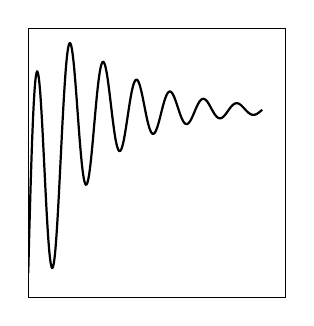
\begin{tikzpicture}
		\begin{axis}[
		name=plot1,
		xmin=0,
		ymax=1.5,
		xtick = \empty,    ytick = \empty,
		y label style = {at={(0,1)},rotate=-90,anchor=south},
		height=5cm,width=\linewidth*0.4
		]
		\addplot[color=black,smooth,thick,-] [samples=500,domain=0:360] {(1-exp(-x/30))+(sin(7*x)*(exp(-x/100)))};;
		\end{axis}
		\end{tikzpicture}
		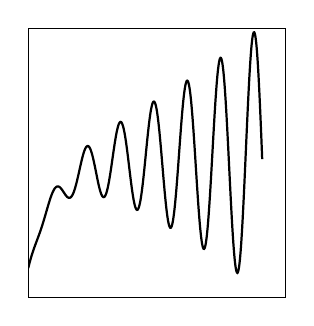
\begin{tikzpicture}
		\begin{axis}[
		name=plot2,
		right of = plot1,
		xmin=0,
		ymax=2.2,
		xtick = \empty,    ytick = \empty,
		height=5cm,width=\linewidth*0.4
		]
		\addplot[color=black,smooth,thick,-] [samples=500,domain=0:360] {(1-exp(-x/40))+(1-exp(x/450))*sin(7*x)};
		\end{axis}
		\end{tikzpicture}
		\begin{tikzpicture}
		\begin{axis}[
		name=plot3,
		at=(plot2.west),
		xmin=0,
		ymax=2.2,
		xtick = \empty,    ytick = \empty,
		height=5cm,width=\linewidth*0.4
		]
		\addplot[color=black,smooth,thick,-] [samples=500,domain=0:360] {(1-exp(-x/40))+(1-exp(-x/80))*sin(7*x)};
		\end{axis}
		\end{tikzpicture}
	\end{minipage}
	\caption{Vrste odziva na skočno spremembo: stabilno, nestabilno, na meji stabilnosti}
\end{figure}
\subsection{Generator trajektorije}
Pozicionirni sistem vsebuje poleg regulacijskih zank še generator trajektorije (angl. Motion Controller). Njegova vloga je podajanje želinih vrednosti pozicije na nadzorovan način s parametri hitrosti in pospeški pomika. Regulacijski krog brez nadzorovane trajektorije, bi se zelo burno odzval, saj bi razlika med želeno in dejansko pozicijo pomenila velik pogrešek, katerega bi regulacijski krog želel nemudoma odpravit. Takšen pogon bi pospešil z največjim možnim pospeškom in se pričel približevati ciljni poziciji z največjo možno hitrostjo ter bi se na cilju zaustavil s prenihajem, kar je tipičen pojav za regulacijski krog s hitrim dinamičnim odzivom. Zahteve po nadzarovanem pomiku so pripeljale do uvedbe generatorja trajektorije. To je algoritem, ki na podlagi vhodnih parametrov ciljne pozicije, zadane hitrosti pomika ter pospeška/pojemka, vnaprej preračuna potek pomikanja. Regulacijski krog poskrbi, da pogon dejansko sledi zadani trajektoriji in odpravlja morebitna odstopanja.\\
Kot primer se lahko vzame načrt leta. Letalo bo ob določeni uri vzleta poletelo iz točke A in pristalo v točki B ob uri pristanka. Po vzletu, pilot s svojim krmarenjem odpravlja zamik smeri, ki jih pozročajo vetrni sunki. Periodično ugotavlja trenutno pozicijo letala in jo primerja z zadanim načrtom poleta ter v primeru odstopanja poveča ali zmanjša hitrost letala do te mere, da pristane točno ob določeni uri pristanka. V primerjavi s pozicionirnim sistemom je pilot regualcijki krog, načrt poleta pa generator trajektorije. Vsakršno odstopanje od zadane trajektorije leta ne vpliva na načrt poleta, saj je ta že vnaprej določen.
Najenostavnejša oblika trajektorje je trapezni profil hitrosti. Pogon najprej pospešuje s konstantnim pospeškom, sledi interval konstantne hitrosti in nato konstantno pojemanje do ciljne pozicije (slika \ref{Trajekt_Trapez}).\\
\begin{figure}[h]
	\centering
	\begin{tikzpicture}
	\begin{axis}[
	xmin=0,
	xmax=5,
	ymin=-1.5,
	ymax=1.5,
	xtick = \empty,    ytick = \empty,
	xlabel = {$t$},
	axis x line=middle,
	%x label style = {at={(1,0)},anchor=west},
	ylabel = {$a, v, s$},
	y label style = {at={(0,1)},rotate=-90,anchor=south},
	%axis lines=left,
	%enlargelimits=1.0,
	legend entries={hitrost,
	pot,
	pospešek},
	legend pos=outer north east]
	\addlegendimage{no markers,black}
	\addlegendimage{no markers,green}
	\addlegendimage{no markers,red}
	\addplot[color=black,smooth,thick][domain=0:1] {(x)};
	\addplot[color=black,smooth,thick][domain=1:3] {(1)};
	\addplot[color=black,smooth,thick][domain=3:4] {-(x-4)};
	\addplot[color=green,smooth,thick][domain=0:1] {(x^2/2)/2};
	\addplot[color=green,smooth,thick][domain=1:3] {(x-0.5)/2};
	\addplot[color=green,smooth,thick][domain=3:4] {(-(x-4)^2/2+3)/2};
	\draw[red,thick] (axis cs:0,0) -- (axis cs:0,0.5) -- (axis cs:1,0.5) -- (axis cs:1,0);
	\draw[red,thick] (axis cs:3,0) -- (axis cs:3,-0.5) -- (axis cs:4,-0.5) -- (axis cs:4,0);
	\end{axis}
	\end{tikzpicture}
	\caption{Trapezni profil hitrosti}
	\label{Trajekt_Trapez}
\end{figure}
Ker je pospešek vzrok navora, kateri je premosorazmeren toku $M\propto I_q $, sledi logično sklepanje, da je sprememba pospeška premosorazmerna spremembi toka skozi čas $\dfrac{da}{dt}\propto \dfrac{di_q}{dt}$. Zaradi induktivnosti navitja motorja, se tok ne more skokovito spreminajati, temveč samo zvezno. V primeru uporabe trapeznega profila hitrosti, ni upoštevana omejitev maksimalne možne spremembe toka skozi čas, zato pogon ne zmore točno sledti temu profilu hitrosti ker že v osnovi ne  upošteva fizikalne omejitve pogona. Takšen način pozicioniranja se uporablja pri nezahtevnih pomikih, saj pogon pri pospeševanju vedno kasni, pri pojemanju pa vedno prehiteva zadano trajektorijo.\\
Rešitev je oblika trajektorije, katera upošteva zgoraj omenjena dejstva in generira hitrost z omejeno spremembo pospeška skozi čas (slika \ref{Trajekt_skriv}). Odvod pospeška po času $j$ (angl. jerk, nem. Ruck) v slovenskem jeziku nima določenega imena, zato ga bom v nadaljevanju imenoval kar sunek, ker se mi zdi to najbolj primeren izraz. Angleški izraz prihaja iz sveta avtomobilizma; izkušen voznik zna mehko speljevati in ne povzroča sunkovitih trzljajev značilnih pri začetniku (angl. jerk driver). Nemški izraz pa že sam po sebi pove, da gre za veličino ki pomeni sunek, oz. koliko pogon "rukne" pri speljevanju.\\
Zaradi omejevanja sunka nastane profil hitrosti bolj mehek in ima  obliko črke S, zato se tudi imenuje S-profil hitrosti.
\begin{equation} \label{Trajekt_ruk}
j(t)=\dfrac{da}{dt}=\dot{a}=\dfrac{d^2v}{dt^2}=\ddot{v}=\dfrac{d^3s}{ds^3}=\dddot{s}
\end{equation}
\begin{figure}[h]
	\centering
	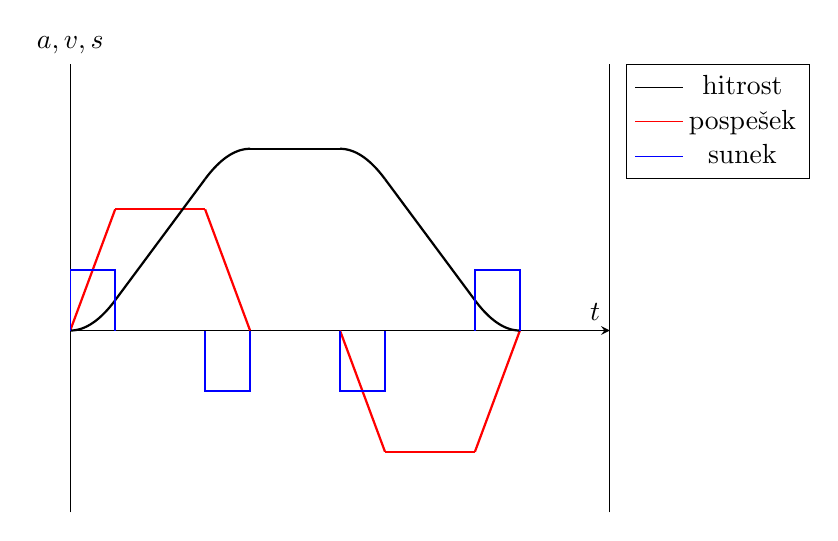
\begin{tikzpicture}
	\begin{axis}[
	xmin=0,
	xmax=12,
	ymin=-1.5,
	ymax=2.2,
	xtick = \empty,    ytick = \empty,
	xlabel = {$t$},
	axis x line=middle,
	%x label style = {at={(1,0)},anchor=west},
	ylabel = {$a, v, s$},
	y label style = {at={(0,1)},rotate=-90,anchor=south},
	%axis lines=left,
	%enlargelimits=1.0,
	legend entries={hitrost,
		pospešek,
		sunek},
	legend pos=outer north east]
	\addlegendimage{no markers,black}
	\addlegendimage{no markers,red}
	\addlegendimage{no markers,blue}
	\addplot[color=red,smooth,thick][domain=0:1] {(x)};
	\addplot[color=red,smooth,thick][domain=1:3] {(1)};
	\addplot[color=red,smooth,thick][domain=3:4] {-(x-4)};
	
	\addplot[color=red,smooth,thick][domain=6:7] {-(x-6)};
	\addplot[color=red,smooth,thick][domain=7:9] {(-1)};
	\addplot[color=red,smooth,thick][domain=9:10] {(x-10)};
	
	\addplot[color=black,smooth,thick][domain=0:1] {(x)^2/2)/2};
	\addplot[color=black,smooth,thick][domain=1:3] {((x-1)+0.5)/2};
	\addplot[color=black,smooth,thick][domain=3:4] {(-(x-4)^2/2+3)/2};
	\addplot[color=black,smooth,thick][domain=4:6] {(3)/2};
	
	\addplot[color=black,smooth,thick][domain=6:7] {(-(x-6)^2/2+3)/2};
	\addplot[color=black,smooth,thick][domain=7:9] {(-(x-7)+2.5)/2};
	\addplot[color=black,smooth,thick][domain=9:10] {((x-10)^2/2)/2};
	
	\draw[blue, thick] (axis cs:0,0) -- (axis cs:0,0.5) -- (axis cs:1,0.5) -- (axis cs:1,0);
	\draw[blue, thick] (axis cs:3,0) -- (axis cs:3,-0.5) -- (axis cs:4,-0.5) -- (axis cs:4,0);
	\draw[blue, thick] (axis cs:6,0) -- (axis cs:6,-0.5) -- (axis cs:7,-0.5) -- (axis cs:7,0);
	\draw[blue, thick] (axis cs:9,0) -- (axis cs:9,0.5) -- (axis cs:10,0.5) -- (axis cs:10,0);
	
	\end{axis}
	\end{tikzpicture}
	\caption{S-profil hitrosti}
	\label{Trajekt_skriv}
\end{figure}
Načeloma se lahko smatra, da je trajektorija že vnaprej preračunana pred vsakim pomikom pogona, vendar v praksi to ni izvedljivo, ker bi bila potrebna velika količina spomina in procoesorskega časa. Trajektorija se preračunava sproti na rekurziven način, v določenih časovnih presledkih, ki so ponavadi daljši od časa vzorčenja regulacijskega kroga. V pozicionirnem sistemu, kjer je prisotnih več pogonskih osi, se ponavadi pojavlja želja tudi po sinhroniziranem pomiku le-teh. Algoritem najprej uskladi pospeške in hitrosti posameznih osi, nato za vsako os generira svojo trajektorijo. Takšni sistemi so CNC obdelovalni stroji. Dodatna vloga generatorjev trajektorij pa je tudi normiranje veličin in kinematična preslikava. Enote hitrosti in pomika so lahko poljubne, pravtako je lahko več osi medseboj povezanih v kompleksen kinematični sklop, ki potrebuje preslikavo iz koordinatnega sistema sklopa v koordinatni sistem osi in obratno.\\
Zaradi svoje velike kompleksnosti izračuna se ti algoritmi trajektorij v praksi večinoma izvajajo na PC platformi. Želene vrednosti hitrosti in pozicije se nato pošiljajo po industrijski komunikaciji (Ethercat, Profinet, Profibus, Sercos) do krmilnih enot pozameznih pogonov. Visoka hitrost prenosa je zaželjena, ni pa najpomembnejša stvar. Zaradi potrebe po sinhronem pomiku več osi, je potreba tudi po obliki sinhrone komunikacije. Vse zgoraj opisane industrijske komunikacije so serijske, PC računalnik pošilja želene in bere dejanske vrednosti zaporedno od prvega do zadnjega pogona povezanih v omrežju, zato bi nastalo do časovnega zamika odziva posameznih osi. Rešitev je poseben protokol komunikacije, ki se mu pravi izohroni (angl. isochronous) prenos podatkov. Vsako stanje je zajeto v točno določenim trenutku s pomočjo ure realnega časa, ki je vgrajena v vsaki napravi. Vse naprave ob točno določenem času naredijo posnetek trenutnega stanja ter hkrati aktivirajo želene vrednosti. 

\chapter{Praktična realizacija krmiljenja pomika in odreza žage s Simotion/Sinamics}
\subsection{Uvod}
Potrebno je bilo realizirati žago katera pomika deske na nastavljeno dolžino in jih odreže z nastavljeno hitrostjo rezanja. Uporabljen je krmilniški sistem Simotion proizvajalca Siemens s servo pogoni Sinamics S120 istega proizvajalca.\\
Simotion je industrijski krmilnik, kateri ima poleg klasičnih funkcij industrijskega krmilnika tudi zmožnost generiranja trajektorij pomikov, ustrezne za podajanje natančne in kontrolirane želene vrednosti poti in hitrosti servo pogonov. Sinamics je družina servo pogonov, zajema krmilno enoto pogona(ov) s komunikacijskim vmesnikom za povezavo s krmilnikom.\\
Žaga je postavljena v liniji strojev za obdelavo lesa. Pred njo se nahaja skener, ki poslika desko iz vseh smeri v vidni in infrardeči svetlobi ter z rentgenskimi žarki. Desko se računalniško analzira in določi reze z namenom odstranitve nezdravih oz. poškodovanih delov deske, kot so grče, vozli in morebitni zaraščeni kovinski ostanki granat (šrapneli). Skener sporoča položaj rezov prek komunikacije TCP/IP krmilniku Simotion. Pred žago se deske nabirajo druga ob drugi in se jih posamićno potiska v stroj, kjer se deska razreže. Slabe kose manjših dimenzij se odstrani s pomočjo izpihovanja, večje pa  s pnevmatskim izmetalom, dobri kosi gredo naprej v naslednji stroj po tekočem traku.

\begin{figure}[h]
	\centering
	\resizebox{\textwidth}{!}{%
		
		\begin{tikzpicture}
		\draw [ thick, rounded corners=5pt]  (5,-1) rectangle (7,-3);
		\draw[black,radius=0.9](3,2) circle; 
		\draw[black,radius=0.9](1,2) circle; 
		\draw[black,radius=0.9](-1,2) circle; 
		\draw[black,radius=0.9](-3,2) circle;
		\draw[black,radius=0.9](-5.5,2) circle;
		\draw[black,radius=0.9](-7.5,2) circle;   
		\draw[black,radius=0.9](10,1.5) circle;   
		\draw[black,radius=0.9](10,4.5) circle;   
		
		\draw[black,radius=0.6](3,4) circle; 
		\draw[black,radius=0.6](1,4) circle; 
		\draw[black,radius=0.6](-1,4) circle; 
		\draw[black,radius=0.6](-3,4) circle;
		\draw[black,radius=0.6](-5.5,4) circle;
		\draw[black,radius=0.6](-7.5,4) circle;   
		
		\draw [ thick, fill=black]  (-4.1,-2.7) rectangle (-4.3,2.7) node[midway, left]{žagin list};
		\draw []  (-4,0) rectangle (-3.9,-6) node[ left]{ekscentričen pomik};
		\draw []   (-3.8,-6) rectangle (-3.7,-4);
		\draw [fill=black]   (-3.9,-6) rectangle (-3.8,-5.8);
		\draw []  (-3.7,-4) rectangle (-3,-4.2);
		\draw [ thick, rounded corners=5pt]  (-3,-5) rectangle (-2,-3.2);
		\draw [ thick]  (-2,-4.7) rectangle (0,-3.6);
		\draw[-,black, ultra thick](10,4.5) -- (14,2) ;
		\draw[black,radius=0.9, fill=white](10,4.5) circle;      
		\pic {gears={size 1 at (6,-2) and size 4 at (6,2)}};
		\pic {gears={size 1 at (3,2) and size 1 at (6,2)}};
		\pic {gears={size 1 at (1,2) and size 1 at (3,2)}};
		\pic {gears={size 1 at (-1,2) and size 1 at (1,2)}};
		\pic {gears={size 1 at (-3,2) and size 1 at (-1,2)}};
		\pic {gears={size 1 at (-5.5,2) and size 1 at (-3,2)}};
		\pic {gears={size 1 at (-7.5,2) and size 1 at (-5.5,2)}};
		\pic {gears={size 1 at (10,1.5) and size 1 at (6,2)}};
		\node[] at (6,-3.5){Motor valjev};
		\node[] at (6,3){jermenica};
		\node[] at (0,0.5){valji pomika desk};
		\node[] at (0,5){odmični pritisni valji};
		\node[] at (12,5){potisno kolo};
		\node[align=center] at (-1,-6){motor pomika žage \\z reduktorjem};
		%\draw[->,>=stealth',semithick] (6:1.2cm) arc[radius=1.2, start angle=150, end angle=210];
		\draw[<->]  ([shift=(-20:5.5)]6,2) arc (-20:10:5.5);
		\draw[<->]  ([shift=(140:6)]14,2) arc (140:160:6);
		\end{tikzpicture}
	}
	\caption{\label{zaga_delovanje} Prikaz delovanja}
\end{figure}
\subsection{Izbira motorjev}
Na sliki \ref{zaga_karakteristike} je prikazana splošna karakteristika servo motorja. Na prvi pogled je takoj vidna podobnost s karakteristiko enosmernega motorja (slika \ref{DcMotor_karaktersitika}). Črtkane črte predstavljajo različno konstrukcijo statorskega navitja. Motor iste velikosti lahko doseže višjo hitrost prostega teka in manjši nazivni navor ali pa nižjo hitrost prostega teka in višji nazivni navor. Podobno kot pri enosmernem motorju ima tudi tukaj vlogo generatorska napetost, ki se veča z številom vrtljajev motorja dokler ne doseže napajalno napetost. Višje hitrosti je možno dosegati v režimu slabljenja polja, kar krmilna enota družine Sinamics S120 tudi premore.\\
Zgornja črna črta $M_{max}$ predstavlja limito maksimalnega mehanskega navora, ki bi povročil poškodbo rotorja zaradi prevelike sile. Violična črta $M{max inv}$ predstavlja maksimalen razpoložljiv navor, ki ga motor lahko ustvari z uporabo pripadajočega močnostnega modula. Rdeča črta $S1(100K)$ je mejna vrednost navora v načinu trajnega obratovanja. Pri pravilni uporabi motorja se  povprečna obremenitev skozi čas mora nahajati pod rdečo krivuljo. 
\begin{figure}[h]
	\centering
	\includegraphics[width=0.8\columnwidth]{S120_karakteristika.jpg}
	\caption{\label{zaga_karakteristike}Karakteristike servo motorjev}
\end{figure}

Motorji so bili izbrani s pomočjo programa Sizer. Za določen sklop je potebno izbrati tip mehanskega sklopa: dvigalo, linearni pomik, valjčni transporter, verižni transporter, ekscentrični pomik, tekoči trak,...Nato je potrebno vpisati prestavna razmerja menjalnika, jermenic, vztrajnostne momente rotirajočih mas, naklon pomika in maso (slika \ref{zaga_sizermeh}).\\
\begin{figure}[h]
	\centering
	\includegraphics[width=1.0\columnwidth]{SizerMechData.jpg}
	\caption{\label{zaga_sizermeh} Vnos mehanskih podatkov}
\end{figure} 
\begin{figure}[h]
	\centering
	\includegraphics[width=1.0\columnwidth]{SizerProfile.jpg}
	\caption{\label{zaga_sizerizhod} Izračunana karakteristika obremenitve/delovanja}
\end{figure}
Sledi želen profil pomika s podatki o pospešku, sunku, hitrosti, potjo in številu zaporednih pomikov. Sizer nato predlaga najbolj ustrezen motor in močnostni krmilni modul ter tudi izriše obratovalno karakteristiko (slika \ref{zaga_sizerizhod}). Ko so bile vstavljene obe osi, je sledil avtomatski izračun napajalnega modula in vse dodatne opreme, kot so kabli, konektroji, dušilke.
\subsection{Napajalni modul}
Izbran napajalni modul je Sinamics Smart Line Module 6SL3130-6TE21-6AA4. To usmernik iz trifazne izmenične napetosti v enosmerno napetost za napajanje motorskih močnostnih modulov. Obratovalna napetost se lahko giblje med 380V in 480V, nazivna moč pa je 16kW. Posebnost taga modula je dvosmerno delovanje in je tako usmernik/razsmernik saj lahko vrača energijo nazaj v omrežje. Motorji pri zaviranju preidejo v generatorski režim obratovnja in vračajo kinetično energijo vrtečih se mas. Klasični trifazni usmerniki, ki temeljijo zgolj na diodnih mostičih nimajo možnosti dvosmernega delovanja, zato potrebujejo dodatne zaviralne upore na katerih se ta povratna energija potroši in gre v izgubo. V sistemu kjer so velike vztrajnosti in veliko dinamičnih pomikov, bi to predstvljalo velik delež izgubne moči, poleg tega pa še nastane težava pri zagotavljanju ustreznega hlajenja zaviralnih uporov. Dvosmerni napajalni modul reši te težave, pojavi pa se tudi potreba po obvezni namestitvi dušilke. Omrežje ima zelo nizko impedanco in bi se za razsmernik obnašalo kot kratek stik, zato je  uporaba dušilke nujna da lahko razsmernik s pomočjo pulzno-širinske modulacije vsili želen tok v omrežje. Napajalni modul se pravtako ne sme nikoli odklopiti od omrežja v času vračanja energije zato ima v ta namen digitalen vhod, kjer se priključi pomožni kontakt glavnega stikala ali odklopnika, kateri mora sprožiti signal nekaj 10ms preden močnostni kontakti dejansko odklopijo omrežno napetost (slika \ref{zaga_napajlnik}).\\
\begin{figure}[htb]
	\centering
	\includegraphics[width=1.0\columnwidth]{SmartLineModule.jpg}
	\caption{\label{zaga_napajlnik} Vezava napajalnega modula \cite{S120PowerModule}}
\end{figure}
\subsection{Valji pomika deske}
Gred motorja poganja jermenski prenos s prestavnim razmerjem $1:4,8$, le-ta pa poganja aluminjaste valje premera $120mm$, ki so med seboj povezani z jermeni. Zastavljeni parameteri pomika so sledeči: maksimalna hitrost $5m/s$, maksimalen pospešek/pojemek $30m/s^2$. Zlasti težaven je bil izbor motorja, ker se z večanjem jermenice povečuje tudi njen vztrajnostni moment, preslikan vztrajnostni moment valjev pa zmanjšuje. Pri nižjem prestavnem razmerju pa se zmanjšuje vztrajnostni moment jermenice, povečuje se premer gnanih valjev in s tem tudi njihov vztrajnostni moment. Premer jermenice $d$, pričvrščene na gred motorja ne sme biti premajhen, ker se radialna sila $F_r=\dfrac{2M}{d}$ povečuje z manjšanjem premera pri enakem izhodnem momentu $M$ motorja. Radialna sila deluje na izhodni ležaj motorske gredi in ne sme biti večja od deklarirane dovoljene radialne sile, sledi $d_{min}=\dfrac{2M_{max}}{F_{r_{max}}}$. Pri večanju prestavnega razmerja jermenic, se na manjši jermenici zmanjšuje površina, ki jo obdaja jermen ter nastaja večja možnost zdrsa jermena. V praksi se je izkazalo, da je jermenski reduktor zelo omejen glede izbire možnega razpona prestavnega razmerja, to dejstvo potrjujejo tudi kombinacije velikosti jermenic, ki jih je možno dobiti na tržišču. 
Pridobljeno razmerje jermenice $1:4,8$, premer valjev $120mm$ ter izbrana nazivna hitrost motorja $3000 o/min$ so bili rezultat izračunov preslikave vztrajnostnih momentov na stran motorja v obliki excel tabele. Šele kasneje so se vrednosti potrdile z vnosom v program Sizer.\\
Tip izbranega motorja za pogon valjev je 1FT7086-5SF71-1NA0 iz serije visoko dinamičnih motorjev s prisilnim zračnim hlajenjem. Ima vgrajen Sin/Cos enkoder s komunikacijskim vmesnikom DriveCliq. Pripadajoči močnostni modul je: 6SL3120-1TE23-0AA4.
\subsection{Pozicijska zanka}
\begin{figure}[h]
	\begin{tikzpicture}[auto, node distance=2cm,>=latex']
	
	\node [input, name=input] {};
	\node [Filt block = {$T_f[s]$}, right of=input, minimum size = 1.5cm, node distance=3cm] (Filter) {};
	\node [sum, right of=Filter,  node distance=2cm] (eps_p) {};

	\node [Pctrl block = {$K_p[s^{-1}]$}, right of=eps_p, minimum size = 1.5cm, node distance=2.5cm] (PosReg) {};
	\node [sum, right of=PosReg, node distance=2cm] (eps_v) {};
	\node [Limit block = {$\Omega_{max}$}, right of=eps_v, minimum size = 0.8cm, node distance=1.5cm] (limita) {};
	\node [output, right of=limita, node distance=2cm] (output) {};
	\node [input, below of=output, node distance=3cm] (dajPos) {};
	
	\draw [draw,->] (input) -- node[at start] {$\Theta_{traj}[rad]$} (Filter);
	\draw [->] (Filter) -- node[name=a] {} (eps_p);		
	\draw [->] (eps_p) -- node {$\varepsilon_{\Theta} $} (PosReg);

	\draw [->] (PosReg) -- node[name=b] {$\Omega_{kor}$} (eps_v);	
	\draw [->] (eps_v) -- node [name=c, at end] {$\Omega_{set}[\frac{rad}{s}]$}(output);
	
	\draw [->] (dajPos) -| node[near start,above]{od dajanika pozicije} node[pos=0.95] {$-$} node [near end] {$\Theta_m$} (eps_p);  %od škatle do sumatorja z neg. predzanakom
	
	\node [name=inputOmega, above of=input,node distance=3cm] {};
	\node[mul right = {$k_{vff}=1$}, above of=eps_v] (feedfwd) {}; %točka izhoda, konec puščice ki pride

	\draw [->] (inputOmega) -|node [at start] {$\Omega_{traj}[\frac{rad}{s}]$} (feedfwd);
	
	\draw [->] (feedfwd) -- node[pos=0.95]{$+$}(eps_v);
	\end{tikzpicture}
	\caption{\label{Regulacije_PozZanka}Pozicijska zanka s kasnjenjem in feedforward }
\end{figure}

\subsection{Hitrostna zanka}
\begin{figure}[h]
	\begin{tikzpicture}[auto, node distance=2cm,>=latex']
	
	\node [input, name=input] {};
	\node [Filt block = {$T_f[s]$}, right of=input, minimum size = 1cm, node distance=2cm] (Filter) {};
	\node [sum, right of=Filter,  node distance=1.5cm] (eps_v) {};	
	\node [PIctrl block = {$K_p[\frac{Nms}{rad}],Ti[s]$}, right of=eps_v, minimum size = 1.5cm, node distance=2cm] (VelReg) {};
	\node [Limit block  = {$M_{max}$}, right of=VelReg, minimum size = 0.5cm, node distance=1.5cm] (limita1) {};	
	\node [sum, right of=limita1, node distance=2.5cm] (eps_m) {};
	\node [sum, right of=eps_m, node distance=1cm] (addfrik) {};
	\node [sum, right of=addfrik, node distance=1cm] (adddead) {};
	\node [output, right of=addfrik, node distance=3cm] (output) {};
	\node [input, below of=output, node distance=3cm] (dajPos) {};		
	\draw [draw,->] (input) -- node[at start] {$\Omega_{set}$} (Filter);
	\draw [->] (Filter) -- node[name=a] {} (eps_v);	
	\draw [->] (eps_v) -- node[] {$\varepsilon_{\Omega} $} (VelReg);	
	\draw [->] (VelReg) -- node[near end] {$M_{kor}$} (eps_m);	
	\draw [->] (eps_m) --  (addfrik);
	\draw [->] (addfrik) --  (adddead);
	\draw [->] (adddead) -- node [near end] {$M_{set}[Nm]$}(output);
	\draw [->] (dajPos) -| node[above, near start]{iz dajanika hitrosti} node[pos=0.95] {$-$} node [near end] {$\Omega_m$} (eps_v);  %od škatle do sumatorja z neg. predzanakom
	\node [Difer block ={$\frac{d}{dt}$} , above of=Filter, minimum size = 1cm, node distance=3cm, xshift=0cm] (odvod) {};
	\node [mul above = {$J[kgm^2]$} , right of=odvod, minimum size = 0.3cm, node distance=2.5cm] (vztrajnost) {};
	\draw	[->] ([xshift=1cm]input) |- (odvod.west);	
	\node[mul above = {$F[\frac{Nms}{rad}]$}, above of=vztrajnost, minimum size = 0.3cm, node distance=2cm] (frikcija) {}; %točka izhoda, konec puščice ki pride
	\draw	[->] ([xshift=1cm]input) |-   (frikcija.west);
	\draw [->] (odvod) -- node[name=e]{$\alpha[\frac{rad}{s^2}]$} (vztrajnost);
	\draw [->] (vztrajnost) -| node[near start]{$M_{dinam}$} node[pos=0.95]{$+$}(eps_m);	
	\draw [->] (frikcija) -| node[near start]{$M_{frikcije}$} node[pos=0.95]{$+$}(addfrik);	
	\node [pinstyle, above of = adddead, align=center, yshift=4cm](teza){$M_{teze}$};
	\draw [->] (teza) -- node[pos=0.95]{$+$}(adddead);	
	\end{tikzpicture}
	\caption{\label{Regulacije_HitrZanka}Hitrostna zanka s kasnjenjem}
\end{figure}
\subsection{Momentna zanka}
	\begin{figure}[h]
	\begin{tikzpicture}[auto, node distance=2cm,>=latex']
	
	\node [input, name=input] {};
	
	\node [Limit block  = {$M_{meh_{max}}$}, right of=input, minimum size = 1cm, node distance=1.5cm] (limita1) {};	
	\node [Limit block  = {$M_{P_{max}}$}, right of=limita1, minimum size = 1cm, node distance=1.5cm] (limita2) {};	
	\node [Limit block  = {$M_{i_{max}}$}, right of=limita2, minimum size = 1cm, node distance=1.5cm] (limita3) {};
	\node [mul above = {$k_i^{-1}[\frac{A}{Nm}]$} ,  right of=limita3, node distance=1.5cm] (mulki) {};	
	\node [notch block, right of=mulki, node distance=2cm] (notch1) {};
	\node [notch block, right of=notch1, node distance=1.5cm] (notch2) {};
	\node [notch block, right of=notch2, node distance=1.5cm] (notch3) {};
	\node [bandstop block, right of=notch3, node distance=1.5cm] (banstop) {};		
	
	\node [output, right of=banstop, node distance=2cm] (output) {};
	\node [input, below of=output, node distance=4cm] (dajPos) {};	
	\node [mul left = {$P_{max}$}, below of=limita2, node distance=1.5cm] (mulomega) {};	
	\node [mul right={$k_i[\frac{Nm}{A}]$}, below of=limita3, node distance=1.5cm] (muliq) {};
	\node [input, below of=muliq, node distance=1cm] (idmax) {};
	
	\draw [->] (input) -- node[at start] {$M_{set}$} (mulki);
	\draw [->] (mulki) --  (notch1); 
	\draw [->] (notch1) --  (notch2); 
	\draw [->] (notch2) -- node(z){} (notch3); 
	\draw [->] (notch3) --  (banstop); 
	\draw [->] (banstop) -- node [at end] {$I_{q_{set}}[A]$} (output); 
	
	\node [above of=z, node distance=1cm, align= center]{\shortstack{\scriptsize Pasovno-zaporna in nizkoprepustna\\\scriptsize frekvenčna sita; korekcijski členi}};
	\draw [->] (dajPos) -| node[above, near start]{iz dajanika hitrosti} node [at end, yshift=-0.5cm] {$\Omega^{-1}_m$} (mulomega);  %od škatle do sumatorja z neg. predzanakom
	\draw [->, shorten >= -8pt] (mulomega) --  (limita2);
	\draw[->] (idmax) --  node[below, at start]{$I_{q_{max}}$} (muliq);   
	\draw[->, shorten >= -8pt] (muliq) --(limita3);  
	\end{tikzpicture}
	\caption{\label{Regulacije_Filtri}Predpriprava tokovne zanke}
\end{figure}

\begin{figure}[h]
	\begin{tikzpicture}[auto, node distance=2cm,>=latex']	
	\node [input, name=input] {};
	\node [Limit block = {$I_{q_{max}}$}, right of=input, minimum size = 0.5cm, node distance=1.5cm] (limq) {};
	\node [sum, right of=limq,  node distance=1.5cm] (epsq) {};	
	\node [PIctrl block = {$K_p[\frac{V}{A}],T_i$}, right of=epsq, minimum size = 1.5cm, node distance=2.5cm] (IqReg) {};
	
	\node [output, right of=IqReg, node distance=4cm] (uq) {};
	\node [input, below of=uq, node distance=2cm] (dajiq) {};	
	\draw [draw,->] (input) -- node[at start] {$I_{q_{set}}[A]$} (epsq);	
	\draw [->] (epsq) -- node[] {$\varepsilon_{I_q} $} (IqReg);	
	\draw [->] (IqReg) -- node [name=c, at end] {$U_{q_{set}}[V]$}(uq);	
	\draw [->] (dajiq) -| node[near start,above]{od merilnika toka} node[pos=0.95] {$-$} node [near end] {$I_{q_m}$} (epsq);  %od škatle do sumatorja z neg. predzanakom
	\node[above of = IqReg]{tokovni regulator q-osi (moment)};
	
	
	\node [input, name=inputd, below of=limq, node distance = 5cm] {};
	\node [sum, right of=inputd,  node distance=1.5cm] (epsd) {};	
	\node [PIctrl block = {$K_p[\frac{V}{A}],T_i$}, right of=epsd, minimum size = 1.5cm, node distance=2.5cm] (IdReg) {};
	\node [output, right of=IdReg, node distance=4cm] (ud) {};
	\node [input, below of=ud, node distance=2cm] (dajid) {};	
	\draw [draw,->] (inputd) -- node[at start] {$I_{d_{set}}[A]$} (epsd);	
	\draw [->] (epsd) --  node[]{$\varepsilon_{I_d} $} (IdReg);	
	\draw [->] (IdReg) -- node [ at end] {$U_{d_{set}}[V]$}(ud);	
	\draw [->] (dajid) -| node[near start,above]{od merilnika toka} node[pos=0.95] {$-$} node [near end] {$I_{d_m}$} (epsd);  %od škatle do sumatorja z neg. predzanakom
	\node[above of = IdReg]{tokovni regulator d-osi (vzbujanje)};		
	\end{tikzpicture}	\caption{\label{Regulacije_DQReg}Tokovni regulatorji q in d-osi}
\end{figure}


\chapter{primeri latex}











%**************** LITERATURA ************************
\bibliographystyle{ieeetrslo}
\bibliography{literatura}

%**************** PRILOGE ************************


\appendix

\chapter{Primer kode PID regulatorja} \label{dodatekB}

\small
\begin{verbatim}
double ek, ek1, ek2, uk1, uk2, ZelenaVrednost, DejanskaVrednost;
double Ts, gamma, u_min, u_max;
double Kpu, Tu, Kp, Ti, Td, Tf, cf, ci, cd;
double q0, q1, q2, p1, p2;

//parametri, ki se preračunajo ob inicializaciji
ek1=ek2=uk1=uk2=u=0.0;
Tf = Td/gamma;
cf = Tf/Ts;
ci = Ts/Ti;
cd = Td/Ts;
p1 = -4*cf/(1+2*cf);
p2 = (2*cf-1)/(1+2*cf);
q0 = Kp * (1 + 2*(cf+cd) + (ci/2)*(1+2*cf))/(1+2*cf);
q1 = Kp * (ci/2-4*(cf+cd))/(1+2*cf);
q2 = Kp * (cf*(2-ci) + 2*cd + ci/2 - 1)/(1+2*cf);

// PID algoritem  preračunan ob vsaki prekinitvi
ek2 = ek1;
ek1 = ek;
ek = (ZelenaVrednost - DejanskaVrednost);
uk2 = uk1;
uk1 = u;

u = q0*ek + q1*ek1 + q2*ek2 - p1*uk1 - p2*uk2;
//limita
if   u>u_max u = u_max;
elseif u<u_min u= u_min;

output=u;
\end{verbatim}






\end{document}
